\documentclass[a4paper,svgnames]{scrartcl}
\usepackage{lmodern}
\usepackage{amssymb,amsmath}
\usepackage{ifxetex,ifluatex,colortbl}
\usepackage{fixltx2e} % provides \textsubscript
\ifnum 0\ifxetex 1\fi\ifluatex 1\fi=0 % if pdftex
  \usepackage[T1]{fontenc}
  \usepackage[utf8]{inputenc}
\else % if luatex or xelatex
  \ifxetex
    \usepackage{mathspec}
  \else
    \usepackage{fontspec}
  \fi
  \defaultfontfeatures{Ligatures=TeX,Scale=MatchLowercase}
\fi
% use upquote if available, for straight quotes in verbatim environments
\IfFileExists{upquote.sty}{\usepackage{upquote}}{}
% use microtype if available
\IfFileExists{microtype.sty}{%
\usepackage[]{microtype}
\UseMicrotypeSet[protrusion]{basicmath} % disable protrusion for tt fonts
}{}
\PassOptionsToPackage{hyphens}{url} % url is loaded by hyperref
\usepackage[unicode=true]{hyperref}
\hypersetup{
            pdftitle={Historical Language Comparison with LingPy and EDICTOR},
            pdfauthor={Johann-Mattis List},
            pdfborder={0 0 0},
            breaklinks=true}
\urlstyle{same}  % don't use monospace font for urls
\usepackage[left=2cm,right=2cm,top=3cm,bottom=3cm]{geometry}
\usepackage{color}
\usepackage{fancyvrb}
\newcommand{\VerbBar}{|}
\newcommand{\VERB}{\Verb[commandchars=\\\{\}]}
\DefineVerbatimEnvironment{Highlighting}{Verbatim}{commandchars=\\\{\}}
% Add ',fontsize=\small' for more characters per line
\newenvironment{Shaded}{}{}
\newcommand{\KeywordTok}[1]{\textcolor[rgb]{0.00,0.44,0.13}{\textbf{#1}}}
\newcommand{\DataTypeTok}[1]{\textcolor[rgb]{0.56,0.13,0.00}{#1}}
\newcommand{\DecValTok}[1]{\textcolor[rgb]{0.25,0.63,0.44}{#1}}
\newcommand{\BaseNTok}[1]{\textcolor[rgb]{0.25,0.63,0.44}{#1}}
\newcommand{\FloatTok}[1]{\textcolor[rgb]{0.25,0.63,0.44}{#1}}
\newcommand{\ConstantTok}[1]{\textcolor[rgb]{0.53,0.00,0.00}{#1}}
\newcommand{\CharTok}[1]{\textcolor[rgb]{0.25,0.44,0.63}{#1}}
\newcommand{\SpecialCharTok}[1]{\textcolor[rgb]{0.25,0.44,0.63}{#1}}
\newcommand{\StringTok}[1]{\textcolor[rgb]{0.25,0.44,0.63}{#1}}
\newcommand{\VerbatimStringTok}[1]{\textcolor[rgb]{0.25,0.44,0.63}{#1}}
\newcommand{\SpecialStringTok}[1]{\textcolor[rgb]{0.73,0.40,0.53}{#1}}
\newcommand{\ImportTok}[1]{#1}
\newcommand{\CommentTok}[1]{\textcolor[rgb]{0.38,0.63,0.69}{\textit{#1}}}
\newcommand{\DocumentationTok}[1]{\textcolor[rgb]{0.73,0.13,0.13}{\textit{#1}}}
\newcommand{\AnnotationTok}[1]{\textcolor[rgb]{0.38,0.63,0.69}{\textbf{\textit{#1}}}}
\newcommand{\CommentVarTok}[1]{\textcolor[rgb]{0.38,0.63,0.69}{\textbf{\textit{#1}}}}
\newcommand{\OtherTok}[1]{\textcolor[rgb]{0.00,0.44,0.13}{#1}}
\newcommand{\FunctionTok}[1]{\textcolor[rgb]{0.02,0.16,0.49}{#1}}
\newcommand{\VariableTok}[1]{\textcolor[rgb]{0.10,0.09,0.49}{#1}}
\newcommand{\ControlFlowTok}[1]{\textcolor[rgb]{0.00,0.44,0.13}{\textbf{#1}}}
\newcommand{\OperatorTok}[1]{\textcolor[rgb]{0.40,0.40,0.40}{#1}}
\newcommand{\BuiltInTok}[1]{#1}
\newcommand{\ExtensionTok}[1]{#1}
\newcommand{\PreprocessorTok}[1]{\textcolor[rgb]{0.74,0.48,0.00}{#1}}
\newcommand{\AttributeTok}[1]{\textcolor[rgb]{0.49,0.56,0.16}{#1}}
\newcommand{\RegionMarkerTok}[1]{#1}
\newcommand{\InformationTok}[1]{\textcolor[rgb]{0.38,0.63,0.69}{\textbf{\textit{#1}}}}
\newcommand{\WarningTok}[1]{\textcolor[rgb]{0.38,0.63,0.69}{\textbf{\textit{#1}}}}
\newcommand{\AlertTok}[1]{\textcolor[rgb]{1.00,0.00,0.00}{\textbf{#1}}}
\newcommand{\ErrorTok}[1]{\textcolor[rgb]{1.00,0.00,0.00}{\textbf{#1}}}
\newcommand{\NormalTok}[1]{#1}
\usepackage{graphicx,grffile}
\makeatletter
\def\maxwidth{\ifdim\Gin@nat@width>\linewidth\linewidth\else\Gin@nat@width\fi}
\def\maxheight{\ifdim\Gin@nat@height>\textheight\textheight\else\Gin@nat@height\fi}
\makeatother
% Scale images if necessary, so that they will not overflow the page
% margins by default, and it is still possible to overwrite the defaults
% using explicit options in \includegraphics[width, height, ...]{}
\setkeys{Gin}{width=\maxwidth,height=\maxheight,keepaspectratio}
\IfFileExists{parskip.sty}{%
\usepackage{parskip}
}{% else
\setlength{\parindent}{0pt}
\setlength{\parskip}{6pt plus 2pt minus 1pt}
}
\setlength{\emergencystretch}{3em}  % prevent overfull lines
\providecommand{\tightlist}{%
  \setlength{\itemsep}{0pt}\setlength{\parskip}{0pt}}
\setcounter{secnumdepth}{0}
% Redefines (sub)paragraphs to behave more like sections
\ifx\paragraph\undefined\else
\let\oldparagraph\paragraph
\renewcommand{\paragraph}[1]{\oldparagraph{#1}\mbox{}}
\fi
\ifx\subparagraph\undefined\else
\let\oldsubparagraph\subparagraph
\renewcommand{\subparagraph}[1]{\oldsubparagraph{#1}\mbox{}}
\fi


% set default figure placement to htbp
\makeatletter
\def\fps@figure{htbp}
\makeatother
\setmainfont[Mapping=tex-text,Scale=1.0]{FreeSans}
\setsansfont[Mapping=tex-text,Scale=1.0]{FreeSans}
\setmonofont{DejaVu Sans Mono}

\title{Historical Language Comparison with LingPy and EDICTOR}
\author{Johann-Mattis List}
\date{November 2017}

\usepackage{scrpage2}
\pagestyle{scrheadings}
\ihead{Johann-Mattis List}
\chead{EDICTOR Tutorial}
\ohead{November 2017}
\ifoot{}
\cfoot{\pagemark}
\ofoot{}


\begin{document}
\maketitle
\begin{abstract}
Historical language comparison for the purpose of identifying cognates
and sound correspondences in multilingual wordlists which can later be
used to infer phylogenetic trees can be conveniently carried out in a
framework of \emph{computer-assisted language comparison} (see
http://calc.digling.org), using tools for automatic inference, like
LingPy (http://lingpy.org,
\href{http://bibliography.lingpy.org?key=List2016e}{List and Forkel
2016}, and tools for data annotation and curation, like EDICTOR
(http://edictor.digling.org,
\href{http://bibliography.lingpy.org?key=List2017d}{List 2017}. In this
tutorial, we will guide the users through all important steps ranging
from data preparation, via data curation, to data export.
\end{abstract}


\section*{1 Preliminaries}\label{preliminaries}
\addcontentsline{toc}{section}{1 Preliminaries}

So far, the majority of all work done in historical linguistics is
carried out manually. Even when people use automatic approaches to infer
phylogenetic trees, using sophisticated algorithms, ranging from
distance-based approaches via parsimony frameworks to likelihood
frameworks, the original data fed to the algorithm is based on manually
annotated cognate sets provided by linguistic experts. While it is clear
that complicated tasks like the identification of cognate words are
difficult to fully automate, specifically when it comes to
distinguishing homology due to borrowing (\emph{xenology} in the
biological literature, see
\href{http://bibliography.lingpy.org?key=List2016f}{List 2016}) from
homology due to true inheritance (\emph{cognacy} in the classical
linguistic literature, ibid.), it is also clear that manual annotation
which is not based on consistent frameworks for data curation bears many
shortcomings:

\begin{enumerate}
\def\labelenumi{\arabic{enumi}.}
\tightlist
\item
  Linguists use a large variety of different formats (in fact,
  researchers often come up with their own ad-hoc format when they start
  to prepare wordlists annotated for cognacy), ignoring that
  well-established ways for cognate annotation have been around since
  the 1990ies (e.g.~the ones used in the STARLING package,
  \href{http://bibliography.lingpy.org?key=Starostin2000a}{Starostin
  2000}).
\item
  Even if linguists know the languages under investigation extremely
  well, ad-hoc formats for annotation often lack the flexibility to
  document all steps which lead to a certain decisions. As a result,
  literature for individual cognate sets is barely cited, and both
  outsiders and insiders often do not even know which parts of the words
  asssigned to the same cognate sets are indeed cognate.
\item
  When converting the manually annotated cognate sets into the format
  required for phylogenetic software packages, linguists do rarely make
  use of automated approaches, but rather often type off the data
  manually, which is not only tedious, but also extremely error-prone,
  especially when dealing with larger datasets, not to speak of the fact
  that it often decouples phylogenetic analysis from the original data,
  making it impossible to trace which words contributed to the decisions
  of the phylogenetic algorithms.
\end{enumerate}

These shortcomings in \emph{transparency}, \emph{efficiency}, and
\emph{accuracy} of currently available datasets call for the use of more
consistent frameworks in which data annotation follows strict rules. The
obvious solution is to use specific \emph{interfaces} for data
annotation and curation, which force scholars to be consistent in their
annotation, thus increasing transparency and accuracy of cognate coding.
In addition, since ad-hoc formats are not specialized for the specific
task of data curation we are dealing with in historical linguistics,
specialized interfaces will also greatly increase the efficiency of data
curation and annotation.

A last advantage to be listed in this context is the fact that scholars
who use improved frameworks for cognate coding can profit a lot from
automatic software packages which may help them to carry out certain
tasks in a semi-automatic fashion, e.g., by first searching for cognates
automatically, and then correcting the errors. This again greatly
increases the efficiency of cognate coding, while at the same time it
may even improve the accuracy, since scholars can conveniently compare
automatically inferred cognates with their manually inferred ones, thus
finding cases where they may have committed an error.

The drawback -- at least following from the feedback given by scholars
from personal communication -- is that scholars have to acquaint
themselves with new tools and even acquire few programming skills. While
the EDICTOR tool for cognate annotation does not require any programming
skills, it requires scholars to understand the major design principles
of cognate coding, i.e., the basic framework proposed by the EDICTOR.
Advanced approaches which make use of LingPy or other software packages
to preparse the data require a basic knowledge of the Python programming
language.

Scholars are at times reluctant of taking these efforts, even when it
comes to mastering the minimal requirements of the EDICTOR tool, which
is written in plain JavaScript and can be launched in a simple
webbrowser. While it is clear that not every linguist wants or should
learn Python, it is not clear -- given that linguists conveniently use
software packages, like Endnote or Zotero for reference managment, word
for text-editing, Excel for ad-hoc annotation of data -- why they should
not be able to acquaint themselves with the few largely intuitive
operations required by tools like STARLING or EDICTOR. Linguistics is a
data-driven discipline, and we are entering the digital age. Historical
linguistics can of course be carried out by writing texts in prose that
argue that some languages are related or for the phylogeny of a certain
language family, but if we want to convince our colleagues and also
render our findings in such a way that not only experts can follow our
reasoning, we need to put our methodology on formal grounds, increasing
the transparency of our judgments.

The following tutorial will be divided into two parts. The first parts
requires some basic Python knowledge. By this, we mean that the users
have a freshly installed version of Python3 on their computer (Python2
is not supported for multiple clashes on Mac-systems where the Python
distribution is corrupted with libraries distributed across non-existing
folders), and that they know how to open a terminal and run a Python
script. We also assume that the relevant Python packages, like LingPy,
Segments package (https://github.com/bambooforest/segments), and the
Concepticon API (https://github.com/clld/concepticon-data) have been
installed in \emph{development mode} on the users computer. Instructions
for installation can be found online for all operation systems.

The second part introduces the EDICTOR and does not require any
programming knowledge, apart from the willingness to dive into the major
ideas of the tool, as well as the patience to explore it.

This tutorial is further supplemented by sample files containing data,
and scripts which run the code described here. We illustrate the major
aspects for different language families to emphasize that the tools are
applicable to virtually all language families, although certain aspects
may require further development in the future.

\section*{2 Preparing the Data}\label{preparing-the-data}
\addcontentsline{toc}{section}{2 Preparing the Data}

As mentioned before, linguists who prepare their own collections of
cognate sets for the purpose of phylogenetic reconstruction often come
up with their own, seemingly convenient, formats for data
representation. Judging from our experience, we can say that these
formats usually have huge disadvantages in terms of transparancy and
inter-operability, and we recommend all users to take the time to read
more about the formats underlying LingPy, EDICTOR, but also the
\emph{Cross-Linguistic Data Formats} initiative
(\href{http://bibliography.lingpy.org?key=Forkel2017a}{Forkel et al.
2017}, see http://cldf.clld.org). These formats are to a large degree
compatible, for LingPy and EDICTOR, they are almost identical, and will
be introduced below.

The most obvious failure in data annotation that many scholars commit
when preparing their data in Excel or other spreadsheet software is that
they include multiple different types of information into one cell.
Thus, if a word has a variant, scholars will place it into one cell in
their spreadsheet software and separate the entries by a comma, a colon,
a tilde, a dash, or at times even by a back-slash, often even using all
of these separators inconsistently for the same dataset. A first and
general rule that people creating data must understand and follow, is
that

\textbf{\texttt{1.} Only one type of information should be put into one
cell in a spreadsheet.}

This rule is non-negotiable, as in our experience with a huge number of
differently coded datasets, scholars necessarily make annotation errors,
even if they try to be consistent. Computers are not like humans, and if
you want to profit from computers to ease your work, assume that they
cannot interpret whether you use a comma and a colon without semantic
difference when listing word variants or whether you do it on purpose.
In fact, humans are also unlikely to understand this, unless it was them
who created the data.

A more general rule deriving from this first rule is the rule that

\textbf{\texttt{2.} All information valid for a given analysis needs to
be consistently annotated.}

This means, for example, that, if root alternation is important for your
reconstruction and cognate decisions, you need to think how to model
this in consistent markup. If your data contains reflexes of an
alternating protoform \texttt{*}\emph{ka-} vs. \texttt{*}\emph{ku-}, for
example, it is not sufficient to simply write
\texttt{*ka-\ \textasciitilde{}\ *ku-} and listing the reflexes,
assuming that your readers will understand which reflex stems from which
of the two alternants. Instead, Two proto-forms should be listed, the
variants should be assigned to the correct proto-form from which they
evolve, and the additional information should be given that
\texttt{*}\emph{ka-} and \texttt{*}\emph{ku-} are variants of the same
root. This practice is rarely followed systematically in etymological
dictionaries, and therefore also often disregarded in databases, but it
is clear that it is the only way to transparently list what reflex stems
from which proto-variant. In fact, this is not a matter of a more
computational approach to historical linguistics, but rather a matter of
improving on our common practice in historical linguistics, which has
for too long a time been based on lax guidelines.

\subsection*{2.1 Data Formats in LingPy and
EDICTOR}\label{data-formats-in-lingpy-and-edictor}
\addcontentsline{toc}{subsection}{2.1 Data Formats in LingPy and
EDICTOR}

Following our rule 1, which claims that only one type of information
should be put into one cell, it is clear that the \emph{language x
concept}-format which scholars use most frequently when representing
word list data is not sufficient. This format essentially reserves one
column for one language in the spreadsheet, and one row for one concept.
The language names are given in the first row, and the concept labels
are given in the first column of the spreadsheet.

\begin{table}
\centering
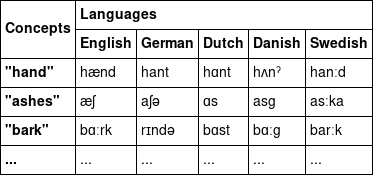
\includegraphics[width=8cm]{images/table-1.png}
\caption{Tabular data format with languages in columns and
concepts in rows.}
\end{table}

This format does not only lack flexibility, as there is only one piece
of information that we can give for each concept ni a given language, it
is also getting more and more impractical if we are dealing with many
different languages, as it will be extremely hard to inspect them on a
screen (scrolling horizontally is always harder for inspection than
scrolling vertically).

Despite the shortcomings, this format, or any variant of it, is one of
the most widespread forms in which language data is annotated nowadays.
The problem of adding essential information on cognacy, or allowing for
synonyms is again mostly handled in an ad-hoc manner. Some scholars add
additional rows for the same concept in order to allow to add more than
one word per meaning and per language (see Table 2).
Some scholars use commata or other separators to add the same entry in
the same cell (Table 3).
And some scholars add another column for the language which shows the
synonym (Table 4).

\begin{table}
\centering
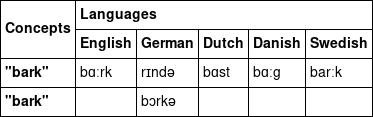
\includegraphics[width=8cm]{images/table-2.png}
\caption{Tabular data format with additional rows for synonym
rendering.}
\end{table}


\begin{table}
\centering
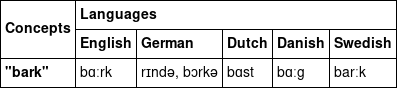
\includegraphics[width=8cm]{images/table-3.png}
\caption{Multiple synonyms in the same cell.}
\end{table}



\begin{table}
\centering
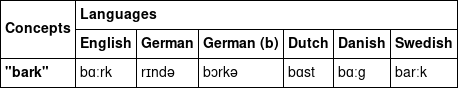
\includegraphics[width=9cm]{images/table-4.png}
\caption{Additional column for language to render synonyms.}
\end{table}

For people concerned with a consistent representation of knowledge, this
is a nightmare, but the nightmare gets even more frightening, when it
comes to the annotation of cognate sets. Here, people have been proving
an incredible amount of phantasy in creating solutions that are
computationally not only difficult to track, but also extremely prone to
errors. Scholars have been using colors (Table 5).
They often even just put the information on cognacy in a separate sheet,
which makes it incredibly difficult to compare their judgments,
especially when then number of language exceeds a handful (Table 6).
At times, they may even binarise the data manually, which is even more
dangerous, as it is almost guaranteed that manually binarising cognate
sets will yield errors (not to speak of the waste of time and the fact
that one cannot trace the characters back when carrying out phylogenetic
analyses, Table 7).


\begin{table}
\centering
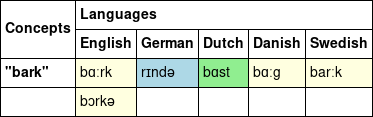
\includegraphics[width=8cm]{images/table-5.png}
\caption{Color-based annotation of cognate sets.}
\end{table}


\begin{table}
\centering
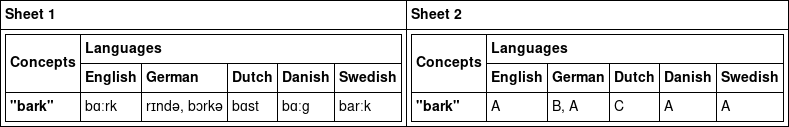
\includegraphics[width=\textwidth]{images/table-6.png}
\caption{Multi-sheet-based annotation of cognate sets.}
\end{table}


\begin{table}
\centering
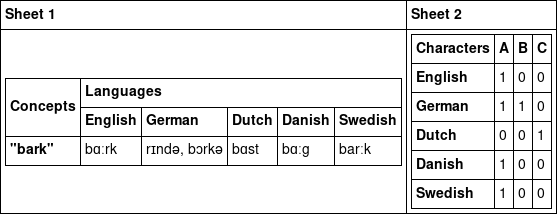
\includegraphics[width=0.75\textwidth]{images/table-7.png}
\caption{Binary annotation of cognate sets in multiple sheets.}
\end{table}

Software packages like STARLING try to circumvent this problem by
allowing for additional columns which add additional information for the
same language. LingPy and EDICTOR, however, employ a different approach
which greatly increases the flexibility of the format. The major
principle of this approach is to reserve one row in the spreadsheet for
exactly one word form. Additional information for each word form is
provided in additional columns (which can be flexibly added by the user
both in LingPy and EDICTOR). The content of each column in a
LingPy/EDICTOR-spreadsheet is given in the header of the file, with the
first column being reserved for a numeric ID which should be greater
than 0 (Table 8).

\begin{table}
\centering
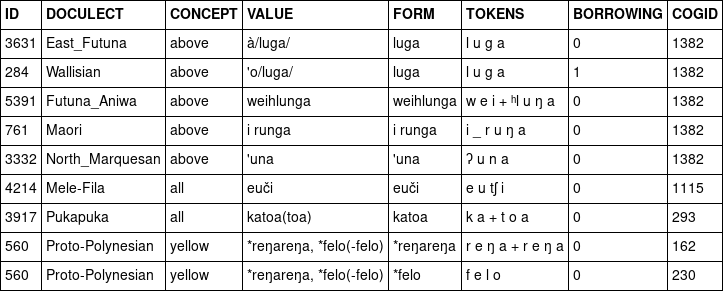
\includegraphics[width=\textwidth]{images/table-8.png}
\caption{Polynesian data example for standard format in LingPy
and EDICTOR.}
\end{table}

While this format seems to be rather redundant on first sight, it offers
a so much greater degree of flexibility that all linguists who started
to seriously test this kind of data representation quickly understand
the advantages. What you need to keep in mind is that the number of
columns is theoretically unlimited. So you can easily add your own
columns which you want to use for either enhanced ways to annotated and
model your data, or to add notes in prose which you can later include in
your publication. You can add sources, and you can be very detailed,
listing the page number for each word form to trace from which source it
was originally taken. The possibilities are virtually unlimited, once
you get a clearer understanding of this way to handle linguistic data.

What is also important to know, in order to understand the superiority
of the representation of data in the way in which it is supported by
EDICTOR and LingPy compared to the ad-hoc format of tabular
representation discussed above, is that the columns are very explicit in
what they require as input. We list eight different columns in our
example, namely \texttt{ID}, \texttt{DOCULECT}, \texttt{CONCEPT},
\texttt{VALUE}, \texttt{FORM}, \texttt{TOKENS}, \texttt{BORROWING},
\texttt{COGID}, but EDICTOR and LingPy allow to add more if needed, and
they do not need all of these columns in order to work properly.

Let us give a brief introduction to the most important aspects regarding
these basic fields (columns) in our example:

\begin{enumerate}
\def\labelenumi{\arabic{enumi}.}
\tightlist
\item
  \textbf{\texttt{ID}}: requires a \emph{unique} numerical value (integer) greater
  than 0, but not necessarily consecutively ordered (i.e., if you have
  5, 10, 10000, all is fine, but you cannot use floats, negative values,
  or 0).
\item
  \textbf{\texttt{DOCULECT}}: requires an arbitrary language name and
  can take virtually any value, but if users plan to export data from
  LingPy and EDICTOR to other formats, users should make sure that their
  language names do NOT include any brackest, spaces, and ideally also
  no other characters than the standard characters from the Latin
  alphabet. Spaces can be conveniently replaced by underscores
  \texttt{\_}, and brackets can be simply deleted. If users insist on
  having specific language names, we recommend to add an additional
  column to their data, where they list the language names as they
  prefer (with brackets and spaces) but that they allow the software to
  deal only with those language names which can be easily exported to
  other data formats.
\item
  \textbf{\texttt{CONCEPT}}: This value can also be arbitrary, but
  ideally, users should avoid inconsistencies. Given that EDICTOR works
  in JavaScript, which means that certain characters may be meaningful
  which are also included in concepts, we recommend to restrict the
  concept labels to alphanumerical entries, ideally not using too many
  brackets, and especially avoiding characters like the
  greater-smaller-sign (\texttt{\textless{}\textgreater{}}) or literal
  quotation marks \texttt{"}.
\item
  \textbf{\texttt{VALUE}}: This column is not required by neither LingPy
  nor EDICTOR, but it is important to show how the data was presented in
  the original source. As you can see in our example, the values are
  considerably modified in the columns \texttt{FORM} and
  \texttt{TOKENS}. For our format, following the specifications
  developed for the CLDF initiative (Forkel et al. 2017), we assume that
  the value is the entry that you find in a source, i.e., a dictionary,
  and that this may consist of multiple forms. As a result, different
  \texttt{FORM}-data for the same concept and the same language may show
  the same value.
\item
  \textbf{\texttt{FORM}}: This column is the single entry extracted from
  a potentially more complex \texttt{VALUE} in a given source. As you
  can see from the last two rows in our example in Table 8, the complex
  value for Proto-Polynesian \emph{yellow} was split into two different
  forms, both being assigned to one row in our data, thus overriding the
  entry given in the original source, the ABVD
  (\href{http://bibliography.lingpy.org?key=Greenhill2008}{Greenhill et
  al. 2008}).
\item
  \textbf{\texttt{TOKENS}}: This is the most important entry for all
  aspects of sequence comparison. It represents the form in both a
  corrected transcription system as well as in \emph{space-segmented
  form}. Scholars have often problems when hearing the first time about
  the segmentation requirement, given that they are confident that they
  can easily guess themselves where the sounds are. However, a computer
  cannot easily do so, especially in ambiguous cases, like affricates
  spelled out with two characters
  (\texttt{\textless{}ts\textgreater{}}), and for this reason, our
  software insists on an unambiguous representation of segments. As an
  additional layer, we allow for a user-defined (as this cannot be
  automated so far) segmentation into morphemes, using the \texttt{+} as
  a marker, as well as a user-defined segmentation into words, using the
  \texttt{\_} as a marker. For morpheme boundaries, linguists often use
  the dash-symbol (\texttt{-}) which we cannot accept since it is
  required to represent gaps in alignment analyses. For word boundaries,
  the space is usually used, which we need to replace by the underscore,
  since the space is already used as a marker for segment boundaries.
\item
  \textbf{\texttt{BORROWING}}: This column is a simple binary column in
  our example which serves the purpose to indicate whether a word has
  been borrowed. More elaborate ways to handle borrowing exist without
  doubt, but for the purpose of turning cognate sets into the binary
  format which is passed to other data formats and fed into phylogenetic
  reconstruction software, the binary format is usually all that is
  needed so far. Users can, however, think of their own ways to provide
  an enhanced codding of borrowings and get in contact with us. If
  sufficient examples are available, we may consider adding it to both
  the LingPy-EDICTOR-formats as well as the CLDF standards.
\item
  \textbf{\texttt{COGID}}: This column is crucial for annotating which
  words are related. The annotation is fairly simple, following the
  STARLING principle as used in older STARLING versions: if two words
  are given the same numeric ID (which must be greater than 0), they are
  judged to be cognate. What is extremely important for users to know is
  that both LingPy and EDICTOR assume that cognate sets are
  \emph{globally} assigned. That is: if you give the same cognate ID to
  words which have different meanings, they will still be regarded as
  cognates. STARLING (in its most recent version which underlies the
  \href{http://starling.rinet.ru/new100/main.htm}{Global Lexicostatistic
  Database},
  \href{http://bibliography.lingpy.org?key=Starostin2011}{Starostin and
  Krylov 2011}) has given up this principle. That means, that
  cross-semantic cognacy can no longer be assigned. Although cognates
  are primarily assigned per meaning class in LingPy and EDICTOR, we are
  trying to develop ideas which allow for improved identification of
  cognates across different meanings. For this reason, we do not allow
  for a \textbf{local identifier}. Problems resulting from the fact that
  identifiers in STARLING need to be (to our knowledge) manually
  assigned and could therefore lead to errors when scholars forget which
  numbers they already used, can be easily avoided when using the
  EDICTOR tool, as it automatically searches for the smallest available
  identifier. Other database projects like
  \href{http://ielex.mpi.nl/}{IELex}
  (\href{http://bibliography.lingpy.org?key=Dunn2012}{Dunn 2012}) use
  alphabetic letters to assign words to cognate sets. We do explicitly
  not follow this practice, as it does not enhance readability and will
  also make the computation of new values for cognate sets much more
  difficult.
\end{enumerate}

If you want to prepare your data in this format to test how it could be
read in by LingPy or EDICTOR, we recommend to start with a spreadsheet
(using Excel, LibreOffice, or GoogleSheets) and inserting the values as
shown above. Once this has been done, you can either export the
spreadsheet to text-format (``csv'', \emph{comma-separated value}), with
a tabstop as delimiter and without quote characters (see the
instructions for this on the web, they are numerous), or, what is often
saver, you copy-paste all columns and cells (only the ones that you
assign, not empty rows or columns should be included!) to an empty text
file which you open with a text-editor of your preference. If you
copy-paste your data in this form, it will automatically be in the
format required by LingPy/EDICTOR.

\subsection*{2.2 Orthography Profiles}\label{orthography-profiles}
\addcontentsline{toc}{subsection}{2.2 Orthography Profiles}

It is probably due to the formulaic attitude to linguistic
reconstruction imposed by
\href{http://bibliography.lingpy.org?key=Saussure1916}{Saussure (1916)}
that linguists often do not seem to worry if they base their
reconstructions on highly inconsistent transcription systems, mixing
various transcription practices with transliteration and even pure
orthography. No matter whether one follows
\href{http://bibliography.lingpy.org?key=Pulgram1959}{Pulgram's (1959)}
skepticism regarding the realism of linguistic reconstruction, or
\href{http://bibliography.lingpy.org?key=Hall1960}{Hall's (1960)}
optimism, for a consistent investigation of linguistic data, the
transcriptions need to be harmonized, and we need to assume that each
segment which is represented as such represents some valid distinction
in a given language. LingPy and EDICTOR offer close support for what
could be called a ``broad version'' of the International Phonetic
Alphabet, that is, they allow for the usage of symbols which are
synonymous, pointing to identical sounds, such as
\texttt{\textless{}ʦ\textgreater{}} vs.
\texttt{\textless{}ts\textgreater{}},
\texttt{\textless{}ʣ\textgreater{}} vs.
\texttt{\textless{}dz\textgreater{}},
\texttt{\textless{}ʧ\textgreater{}} vs.
\texttt{\textless{}tʃ\textgreater{}}, or
\texttt{\textless{}ʤ\textgreater{}} vs.
\texttt{\textless{}dʒ\textgreater{}}, and often going even beyond that,
accepting symbols which are used in alternative transcription
transcriptions, like \texttt{\textless{}č\textgreater{}} or
\texttt{\textless{}ž\textgreater{}}, which are internally treated as
\texttt{\textless{}tʃ\textgreater{}} and
\texttt{\textless{}dʒ\textgreater{}}. Nevertheless, judging from our
experience with both computer-based and computer-assisted language
comparison in the past, we highly recommend to all users to closely
follow the IPA, ideally in the explicit version developed as part of the
\emph{Cross-linguistic transcription systems} initiative (List et al. in
preparation), for which an online demo is available
(http://calc.digling.org/clts/).

If you want to prepare your data adequately, starting from the
\texttt{VALUES}, you have basically three choices: You can (a) prepare
and segment the data manually, by adding spaces and correcting wrong
transcriptions, deleting spaces, splitting values into forms, etc., you
can (b) hope that your data is more or less in a good state and trust
that LingPy automatically segments your data properly enough, and (c)
you can follow a semi-automated workflow in which you use some Python
code to split your values into different forms which you then
automatically segment and modify with help of \emph{orthography
profiles} (\href{http://bibliography.lingpy.org?key=Moran2017}{Moran and
Cysouw forthcoming}).

An orthography profile can be thought of as a simple text file with two
or more columns in which the first represents the values as you find
them in your data (i.e., non-IPA transcriptions, etc.), and the other
columns allowing you to convert the sequence of characters that you find
in the first column. So in brief, you have a source-pattern and a
replacement pattern:

\begin{table}
\centering
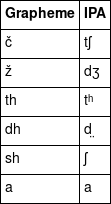
\includegraphics[width=3cm]{images/table-9.png}
\caption{A simple orthography profile.}
\end{table}

If you save this profile in tab-separated form (as explained in the end
of the previous section), you can easily use it to convert all words
which have nothing but the required segments in the profile into the
target transcription (the profile above is provided with this tutorial
as file \texttt{simple-profile.tsv}:

\begin{Shaded}
\begin{Highlighting}[]
\CommentTok{# import relevant modules}
\ImportTok{from}\NormalTok{ segments.tokenizer }\ImportTok{import}\NormalTok{ Tokenizer}

\CommentTok{# load the tokenizer object}
\NormalTok{tk }\OperatorTok{=}\NormalTok{ Tokenizer(}\StringTok{'P_simple-profile.tsv'}\NormalTok{)}

\CommentTok{# convert a string to test it}
\BuiltInTok{print}\NormalTok{(tk(}\StringTok{'čathashadhža'))}
\StringTok{print(tk('}\NormalTok{čathashadhža}\StringTok{', column='}\NormalTok{IPA}\StringTok{'))}
\end{Highlighting}
\end{Shaded}

\begin{verbatim}
č a th a sh a dh ž a
tʃ a tʰ a ʃ a d̤ dʒ a
\end{verbatim}

What you can see from this small example is that the orthography profile
code does essentially two things: it segments the word by treating all
those characters as one segment which you listed in the
\texttt{Grapheme} column, and it can further be used to convert those
segments automatically, in case you provided an additional column (in
our case called \texttt{IPA}).

If your profile is not sufficient to list all relevant characters or
character combinations, however, the code will yield erroneous output:

\begin{Shaded}
\begin{Highlighting}[]
\BuiltInTok{print}\NormalTok{(tk(}\StringTok{'catapura'}\NormalTok{))}
\BuiltInTok{print}\NormalTok{(tk(}\StringTok{'catapura'}\NormalTok{, column}\OperatorTok{=}\StringTok{'IPA'}\NormalTok{))}
\end{Highlighting}
\end{Shaded}

\begin{verbatim}
� a � a � � � a
� a � a � � � a
\end{verbatim}

You can see from this example, that only the ``a'' is recognized as a
valid variant in the string \texttt{catapura}, as the relevant
characters are not given in our profile. As a result, you may imagine
that it is quite tedious to write an initial orthography profile on your
own, specifically when you have not a sound knowledge of the variation
in your data.

To ease the pain, we have written a script that uses LingPy's rather
well-informed algorithm for segmentation and can be used for the initial
creation of orthography profiles. We demonstrate the usage with the
small example file \texttt{P\_input-file.tsv}, which contains a couple
of Germanic languages and only two concepts. The file which LingPy
creates will be called \texttt{P\_profile.tsv}. This code can be run in
any commandline, so in contrast to the Python code above, you only need
to open a terminal, and type in the following commands:

\begin{verbatim}
$ lingpy profile -i P_input-file.tsv -o 
  P_simple-profile.tsv --column=ipa
\end{verbatim}

The resulting profile will look as shown in Table 10.

\begin{table}
\centering
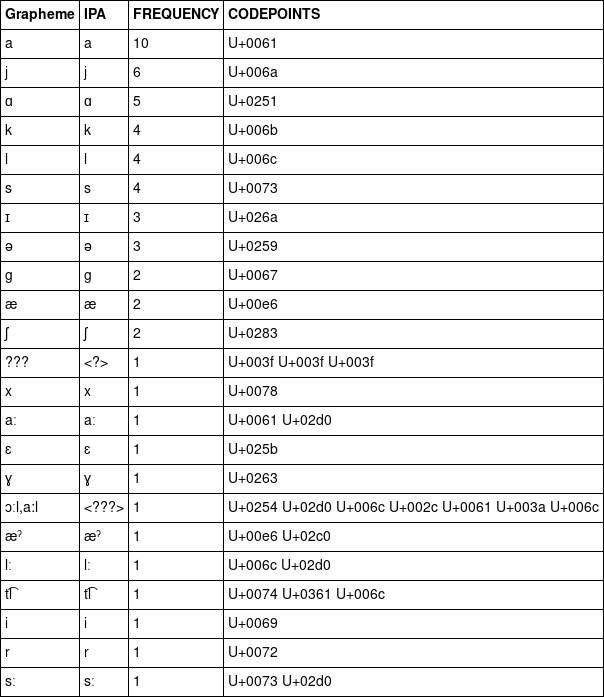
\includegraphics{images/table-10.png}
\caption{Preliminary orthography profile with help of LingPy.}
\end{table}

You can see that in additoin to the IPA column, the code also lists the
frequency and the Unicode codepoints. If the IPA column contains the
character sequence \texttt{\textless{}?\textgreater{}}, it means that
LingPy cannot interprete the sound segment. If it contains the
characters sequence \texttt{\textless{}???\textgreater{}}, it means that
the full entry could not be resolved.

Once having created an initial profile in this way, you can then easily
modify the characters yourself, and apply it to your original data. In
order to illustrate this, we have updated the profile, replacing the
questionable cases as shown in Table 11.

\begin{table}
\centering
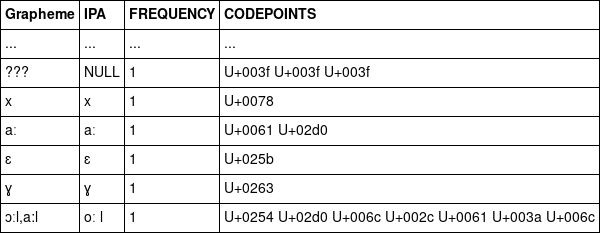
\includegraphics{images/table-11.png}
\caption{Corrected orthography profile.}
\end{table}

Note that in this case, we decided that the \texttt{???} should no
longer be rendered in the data, which is why we replace them by
\texttt{NULL} a specific term used to indicate that something should be
deleted upon conversion. In the other case we decided to take the first
form, and we list only this form, but we manually segment it, following
the basic principle of segmentation which says that sounds which form a
unit should be grouped into one segment each.

With this corrected profile, which you find with the filename
\texttt{P\_modified-profile.tsv}, we can now enhance our data with help
of some short Python code:

\begin{Shaded}
\begin{Highlighting}[]
\ImportTok{from}\NormalTok{ lingpy }\ImportTok{import} \OperatorTok{*}
\ImportTok{from}\NormalTok{ segments.tokenizer }\ImportTok{import}\NormalTok{ Tokenizer}
\NormalTok{wl }\OperatorTok{=}\NormalTok{ Wordlist(}\StringTok{'P_input-file.tsv'}\NormalTok{)}
\NormalTok{op }\OperatorTok{=}\NormalTok{ Tokenizer(}\StringTok{'P_modified-profile.tsv'}\NormalTok{)}
\NormalTok{wl.add_entries(}\StringTok{'tokens'}\NormalTok{, }\StringTok{'ipa'}\NormalTok{, op, column}\OperatorTok{=}\StringTok{'IPA'}\NormalTok{)}
\NormalTok{wl.output(}\StringTok{'tsv'}\NormalTok{, filename}\OperatorTok{=}\StringTok{'P_output-file'}\NormalTok{, ignore}\OperatorTok{=}\StringTok{'all'}\NormalTok{,}
    \NormalTok{prettify}\OperatorTok{=}\VariableTok{False}\NormalTok{)}
\ControlFlowTok{for}\NormalTok{ idx, doculect, form, tokens }\KeywordTok{in}\NormalTok{ wl.iter_rows(}\StringTok{'doculect'}\NormalTok{, }\StringTok{'ipa'}\NormalTok{, }\StringTok{'tokens'}\NormalTok{):}
    \ControlFlowTok{if}\NormalTok{ form }\OperatorTok{!=}\NormalTok{ tokens.replace(}\StringTok{' '}\NormalTok{, }\StringTok{''}\NormalTok{):}
        \BuiltInTok{print}\NormalTok{(}\StringTok{'}\SpecialCharTok{\{0:10\}}\StringTok{ }\SpecialCharTok{\{1:10\}}\StringTok{ }\SpecialCharTok{\{2:15\}}\StringTok{'}\NormalTok{.}\BuiltInTok{format}\NormalTok{(doculect, form, tokens))}
    \end{Highlighting}
\end{Shaded}

\begin{verbatim}
German     ???ɪx      ɪ x            
English    ɔːl,a:l    oː l           
\end{verbatim}

You can see, the profile code has successfully converted the data in the
file, and if you inspect the file \texttt{P\_output-file.tsv} you will
see that an additional column with \texttt{TOKENS} was added to the
file.

There is an enhanced way to make use of orthography profiles, namely by
adding simple context, such as ``occurs in the beginning'' and ``occurs
in the end''. You will need to tweak the code a little bit, but
context-sensitive profiles may come in handy if you deal with more
complex data:

\begin{verbatim}
$ lingpy profile -i P_input-file.tsv -o P_context-profile.tsv --column=ipa 
  --context
\end{verbatim}

The resulting profile has the following appearance:

\begin{table}
\centering
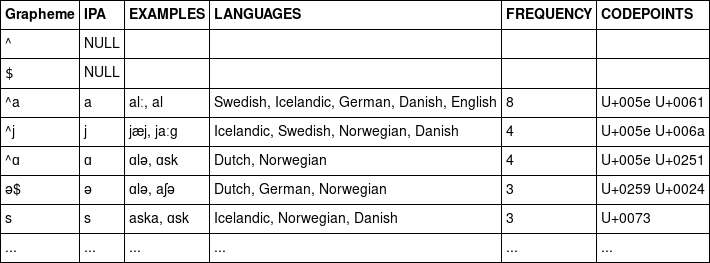
\includegraphics{images/table-12.png}
\caption{Extended orthography profile with context.}
\end{table}

As you can see, the number of rows has slightly increased, since this
time, each character is given at least three times: one time as the
beginning of a word form (marked by the character \texttt{\^{}}), one
time in the middle of a word, and one time as the end of a word form
(marked by the Dollar character \texttt{\$}). The profile is also more
verbose in so fwar as it gives examples and the languages in which these
examples occur. Correcting this profile is a bit more tedious, but it
has the advantage of allowing you to be much more precise in your
conversions. When converting the data with help of Python later, you
must remember to add the start- and end-markers to each sound, which
renders the code a bit more complex (assuming a corrected profile
\texttt{P\_corrected-context-profile.tsv}):

\begin{Shaded}
\begin{Highlighting}[]
\NormalTok{wl }\OperatorTok{=}\NormalTok{ Wordlist(}\StringTok{'P_input-file.tsv'}\NormalTok{)}
\NormalTok{op }\OperatorTok{=}\NormalTok{ Tokenizer(}\StringTok{'P_modified-context-profile.tsv'}\NormalTok{)}
\NormalTok{wl.add_entries(}\StringTok{'tokens'}\NormalTok{, }\StringTok{'ipa'}\NormalTok{, }\KeywordTok{lambda}\NormalTok{ x: op(}\StringTok{'^'}\OperatorTok{+}\NormalTok{x}\OperatorTok{+}\StringTok{'$'}\NormalTok{, column}\OperatorTok{=}\StringTok{'IPA'}\NormalTok{))}
\NormalTok{wl.output(}\StringTok{'tsv'}\NormalTok{, filename}\OperatorTok{=}\StringTok{'P_output-file'}\NormalTok{, ignore}\OperatorTok{=}\StringTok{'all'}\NormalTok{, prettify}\OperatorTok{=}\VariableTok{False}\NormalTok{)}
\ControlFlowTok{for}\NormalTok{ idx, doculect, form, tokens }\KeywordTok{in}\NormalTok{ wl.iter_rows(}\StringTok{'doculect'}\NormalTok{, }\StringTok{'ipa'}\NormalTok{, }\StringTok{'tokens'}\NormalTok{):}
    \ControlFlowTok{if}\NormalTok{ form }\OperatorTok{!=}\NormalTok{ tokens.replace(}\StringTok{' '}\NormalTok{, }\StringTok{''}\NormalTok{):}
        \BuiltInTok{print}\NormalTok{(}\StringTok{'}\SpecialCharTok{\{0:10\}}\StringTok{ }\SpecialCharTok{\{1:10\}}\StringTok{ }\SpecialCharTok{\{2:15\}}\StringTok{'}\NormalTok{.}\BuiltInTok{format}\NormalTok{(doculect, form, tokens))}
\end{Highlighting}
\end{Shaded}

\begin{verbatim}
German     ???ɪx      ɪ x            
English    ɔːl,a:l    oː l           
\end{verbatim}

\subsection*{2.4 Automatic Analysis with
LingPy}\label{automatic-analysis-with-lingpy}
\addcontentsline{toc}{subsection}{2.4 Automatic Analysis with LingPy}

Once you have assembled your data in the form discussed above, it is
straightforward to use LingPy to carry out an initial search for
cognates. Thus, using the file \texttt{P\_output-file.tsv}, we can
easily search for cognates in our data.

\begin{Shaded}
\begin{Highlighting}[]
\NormalTok{lex }\OperatorTok{=}\NormalTok{ LexStat(}\StringTok{'P_output-file.tsv'}\NormalTok{)}
\NormalTok{lex.cluster(method}\OperatorTok{=}\StringTok{'sca'}\NormalTok{, threshold}\OperatorTok{=}\FloatTok{0.45}\NormalTok{, ref}\OperatorTok{=}\StringTok{'cogid'}\NormalTok{)}
\NormalTok{lex.output(}
    \StringTok{'tsv'}\NormalTok{, }
\NormalTok{    filename}\OperatorTok{=}\StringTok{'P_cognate-file'}\NormalTok{, }
\NormalTok{    subset}\OperatorTok{=}\VariableTok{True}\NormalTok{, }
\NormalTok{    prettify}\OperatorTok{=}\VariableTok{False}\NormalTok{, }
\NormalTok{    ignore}\OperatorTok{=}\StringTok{'all'}
\NormalTok{)}
\end{Highlighting}
\end{Shaded}

The resulting file looks as shown in Table 13.

\begin{table}
\centering
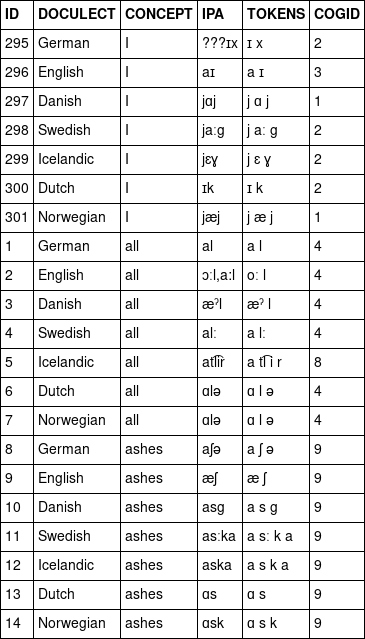
\includegraphics[width=0.7\textwidth]{images/table-13.png}
\caption{Output of automatic cognate detection in LingPy.}
\end{table}

Thus, you can see that LingPy added the \texttt{COGID} column which
contains the automated cognate judgments made by the algorithm we used.

You can also align the data, which can be easily done as follows:

\begin{Shaded}
\begin{Highlighting}[]
\NormalTok{alm }\OperatorTok{=}\NormalTok{ Alignments(lex, ref}\OperatorTok{=}\StringTok{'cogid'}\NormalTok{)}
\NormalTok{alm.align()}
\NormalTok{alm.output(}
    \StringTok{'tsv'}\NormalTok{, }
\NormalTok{    filename}\OperatorTok{=}\StringTok{'P_alignment-file'}\NormalTok{, }
\NormalTok{    subset}\OperatorTok{=}\VariableTok{True}\NormalTok{, }
\NormalTok{    cols}\OperatorTok{=}\NormalTok{[}\StringTok{'doculect'}\NormalTok{, }\StringTok{'concept'}\NormalTok{, }\StringTok{'ipa'}\NormalTok{, }\StringTok{'tokens'}\NormalTok{, }\StringTok{'cogid'}\NormalTok{, }\StringTok{'alignment'}\NormalTok{], }
\NormalTok{    prettify}\OperatorTok{=}\VariableTok{False}\NormalTok{, }
\NormalTok{    ignore}\OperatorTok{=}\StringTok{'all'}
\NormalTok{)}
\end{Highlighting}
\end{Shaded}

The output now looks as shown in Table 14.

\begin{table}
\centering
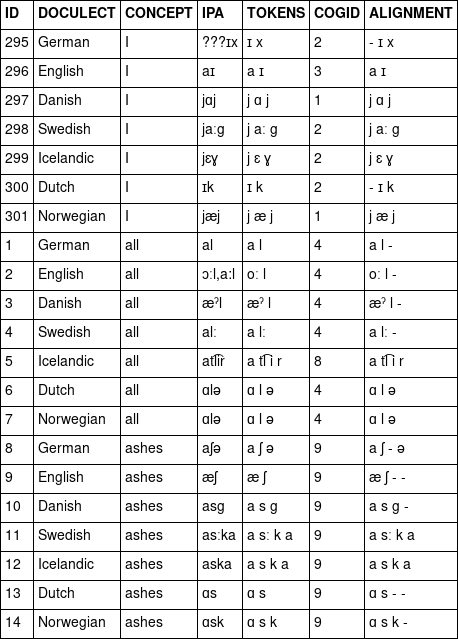
\includegraphics[width=0.75\textwidth]{images/table-14.png}
\caption{Aligned output in LingPy.}
\end{table}

You can see, that LingPy added an \texttt{ALIGNMNENT} column which
essentially has the same structure as the \texttt{TOKENS} with the
difference that it contains aligned data, thus, for each cognate set,
gaps may have been introduced for sounds which do not correspond to any
other sounds. Needless to say that this kind of data is best inspected
with the EDICTOR, where you can then directly start to correct wrong
alignments or cognate sets.

\subsection*{2.5 Enhancing Your Data}\label{enhancing-your-data}
\addcontentsline{toc}{subsection}{2.5 Enhancing Your Data}

You should always be keen on making your data as transparent as
possible. This means as well that you should give other people the
chance to immediately know which concepts you were investigating and
which language varieties. For language varieties, you should provide a
\texttt{languages.csv} file in which you list the name you use in your
dataset for each language variety along with the Glottocode (if you can
find one).

To make sure that your data is comparable in terms of the concepts that
you investigated, you should link your questionnaire to the Concepticon
(\href{http://bibliography.lingpy.org?key=List2016a}{List et al. 2016}).
Many scholars still have a huge problem in understanding what the
Concepticon actually is. We won't go into the details here, but if you
are interested in selecting comparable questionnaires (e.g., words less
prone to borrowing) for your language sample, you should definitely have
a close look at the Concepticon website at http://concepticon.clld.org,
since it is highly likely that your specific questionnaire has already
been linked. In this case, you should download the concept list in the
form in which it is provided by the Concepticon project, as this will
spare you the time of typing it off yourself (which may introduce new
errors), and you will get a lot of meta-information which may be useful.
For example, if you download the Leipzig-Jakarta list
(\href{http://bibliography.lingpy.org?key=Tadmor2009}{Tadmor 2009},
\href{http://concepticon.clld.org/contributions/Tadmor-2009-100}{Tadmor-2009-100}),
you may first learn a lot about how it was constructed, but you can also
directly compare it with lists that may be similar. If you want to know
how stable the concepts in this list are, for example, you could have a
look at the basic list underlying the original project
(\href{http://concepticon.clld.org/contributions/Haspelmath-2009-1460}{Haspelmath-2009-1460}),
where you will receive explicit ranks for all concepts.

If you want to check the overlap between the Leipzig-Jakarta list and
Swadesh's (\href{http://bibliography.lingpy.org?key=Swadesh1955}{1955})
list of 100 items, you can use the Concepticon API, querying for the
intersection of both lists:

\begin{verbatim}
$ concepticon intersection Tadmor-2009-100 Swadesh-1955-100
  1   ARM OR HAND            [2121] HAND (1, Swadesh-1955-100)
  2   ASH                    [646 ] 
  3   BIG                    [1202] 
  4   BIRD                   [937 ] 
  5   BITE                   [1403] 
  6   BLACK                  [163 ] 
  7   BLOOD                  [946 ] 
  8   BONE                   [1394] 
  9   BREAST                 [1402] 
 10   BURN                   [2102] BURNING (1, Tadmor-2009-100)
 11   COME                   [1446] 
 12   DOG                    [2009] 
 13   DRINK                  [1401] 
 14   EAR                    [1247] 
 15   EARTH (SOIL)           [1228] 
 16   EAT                    [1336] 
 17   EGG                    [744 ] 
 18   EYE                    [1248] 
 19   FIRE                   [221 ] 
 20   FISH                   [227 ] 
 21   FLESH OR MEAT          [2615] 
 22   FLY (MOVE THROUGH AIR) [1441] 
 23   FOOT OR LEG            [2098] FOOT (1, Swadesh-1955-100)
 24   GIVE                   [1447] 
 25   GO                     [695 ] WALK (1, Swadesh-1955-100)
 26   GOOD                   [1035] 
 27   HAIR                   [1040] 
 28   HEAR                   [1408] 
 29   HORN (ANATOMY)         [1393] 
 30   I                      [1209] 
 31   KNEE                   [1371] 
 32   KNOW (SOMETHING)       [1410] 
 33   LEAF                   [628 ] 
 34   LIVER                  [1224] 
 35   LONG                   [1203] 
 36   LOUSE                  [1392] 
 37   MOUTH                  [674 ] 
 38   NAME                   [1405] 
 39   NECK                   [1333] 
 40   NEW                    [1231] 
 41   NIGHT                  [1233] 
 42   NOSE                   [1221] 
 43   NOT                    [1240] 
 44   ONE                    [1493] 
 45   RAINING OR RAIN        [2108] RAIN (PRECIPITATION) (1, Tadmor-2009-100)
 46   RED                    [156 ] 
 47   ROOT                   [670 ] 
 48   SAND                   [671 ] 
 49   SAY                    [1458] 
 50   SEE                    [1409] 
 51   SKIN                   [763 ] 
 52   SMALL                  [1246] 
 53   SMOKE (EXHAUST)        [778 ] 
 54   STAND                  [1442] 
 55   STAR                   [1430] 
 56   STONE OR ROCK          [2125] STONE (1, Swadesh-1955-100)
 57   TAIL                   [1220] 
 58   THIS                   [1214] 
 59   THOU                   [1215] 
 60   TONGUE                 [1205] 
 61   TOOTH                  [1380] 
 62 * TREE OR WOOD           [2141] WOOD (1, Tadmor-2009-100), 
                                    TREE (1, Swadesh-1955-100)
 63   WATER                  [948 ] 
 64   WHAT                   [1236] 
 65   WHO                    [1235] 
\end{verbatim}

From this output, you can learn that Leipzig-Jakarta lists ``arm or
hand'' as a concept, while Swadesh is more concrete, listing only
``hand''. You can also learn that Swadesh is not very concrete regarding
the concept ``rain'' where he fails to inform us whether it was intended
as a noun or a verb. From the match 62, you can further see that
``tree'' and ``wood'' are both judged to be subsets of the meta-concept
``tree or wood'', and indeed, there are quite a few languages which do
not distinguish between the two.

There are more possibilities: The \texttt{concepticon\ union} command
allows you to calculate the union of different lists, thus allowing you
to create your own questionnaires based on different concept lists. By
typing the following command in the command line, for example, you can
learn that the union of Leipzig-Jakarta and Swadesh's 100-item list are
135 concepts:

\begin{verbatim}
$ concepticon union Tadmor-2009-100 Swadesh-1955-100 | wc -l
135
\end{verbatim}

And if you add the 200-item list by Swadesh
(\href{http://bibliography.lingpy.org?key=Swadesh1952}{1952}), you will
see that the union has 222 concepts:

\begin{verbatim}
$ concepticon union Tadmor-2009-100 Swadesh-1955-100 Swadesh-1952-200 | wc -l
222
\end{verbatim}

More importantly, if you want to merge data from different
questionnaires or datasets where your do not know to which degree
concepts overlap, you can use the automatic mapping algorithm provided
by the Concepticon API to get a first intelligent guess which concepts
your data contains. This works even across different languages, as we
have so far assembled concept labels in quite a few different language
varieties which we can use to search for similar concepts. The command
is a simple as typing
\texttt{concepticon\ map\_concepts\ \textless{}yourconceptlist\textgreater{}}
in your terminal, where you replace
\texttt{\textless{}yourconceptlist\textgreater{}} with your filename. We
have prepared three files, one in English, one in Chinese, and one in
German, all showing the following tabule structure (the following being
from the file \texttt{C\_concepts.tsv}):

\begin{verbatim}
NUMBER  ENGLISH
1   word
2   hand
3   eggplant
4   aubergine
5   simpsons (tv series)
\end{verbatim}

In order to link this English file to the Concepticon, all we have to do
is to type:
 
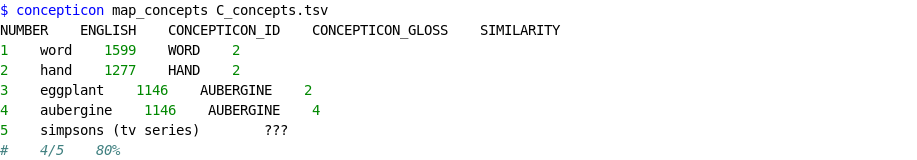
\includegraphics[width=\textwidth]{images/code-1.png}
%\begin{verbatim}
%$ concepticon map_concepts C_concepts.tsv
%NUMBER  ENGLISH CONCEPTICON_ID  CONCEPTICON_GLOSS   SIMILARITY
%1   word    1599    WORD    2
%2   hand    1277    HAND    2
%3   eggplant    1146    AUBERGINE   2
%4   aubergine   1146    AUBERGINE   4
%5   simpsons (tv series)        ??? 
%#   4/5 80% 
%\end{verbatim}

The output tells us first, whether the Concepts can be linked to
Concepticon, and second, it gives us the overall percentage for inferred
links. You can see that the mapping algorithm is not based on simple
string identity, as it correctly links ``eggplant'' to the concept set
\texttt{AUBERGINE}.

Similarly, we can try to link our file with Chinese concepts, the file
\texttt{C\_concepts-chinese.tsv}:
 
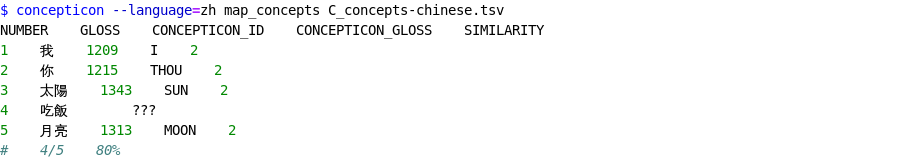
\includegraphics[width=\textwidth]{images/code-2.png}

%\begin{verbatim}
%$ concepticon --language=zh map_concepts C_concepts-chinese.tsv
%NUMBER  GLOSS   CONCEPTICON_ID  CONCEPTICON_GLOSS   SIMILARITY
%1   我   1209    I   2
%2   你   1215    THOU    2
%3   太陽  1343    SUN 2
%4   吃飯      ??? 
%5   月亮  1313    MOON    2
%#   4/5 80% 
%\end{verbatim}

And accordingly also our file \texttt{C\_concepts-german.tsv}:

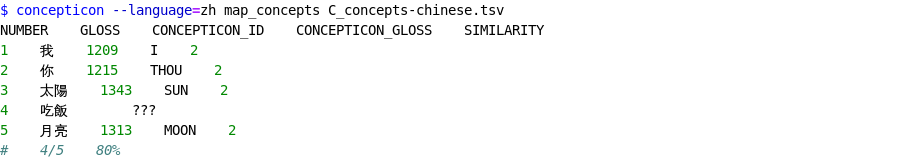
\includegraphics[width=\textwidth]{images/code-2.png}

%\begin{verbatim}
%$ concepticon --language=de map_concepts C_concepts-german.tsv
%NUMBER  GLOSS   CONCEPTICON_ID  CONCEPTICON_GLOSS   SIMILARITY
%1   Hand    1277    HAND    2
%2   Schuh   1381    SHOE    2
%3   Fuß 1301    FOOT    2
%4   Abend   1629    EVENING 2
%5   Sonne   1343    SUN 2
%#   5/5 100%    
%\end{verbatim}

The Concepticon is a collaborative effort that is supposed to render our
linguistic data more comparable. The more questionnaires we can add to
our collection, the easier it will be for future research to build on
these resources. Even if you think that you do not need to link your
data to Concepticon, since you anyway use the ``standard list'' by
Swadesh, you should at least provide a \texttt{concepts.tsv} file in
which you list your explicit links. In this way you guarantee that other
can re-use your data and also contribute to the collaborative efforts
which are currently being done in the context of the CLDF initiative.

\section*{3 Annotating and Data with
EDICTOR}\label{annotating-and-data-with-edictor}
\addcontentsline{toc}{section}{3 Annotating and Data with EDICTOR}

\subsection*{3.1 Overview}\label{overview}
\addcontentsline{toc}{subsection}{3.1 Overview}

The Etymological DICtionary ediTOR (EDICTOR, \url{http://edictor.digling.org},
\href{http://bibliography.lingpy.org?key=List2017d}{List 2017}) is a
free, interactive, web-based tool that was specifically designed to
serve as an interface between quantitative and qualitative tasks in
historical linguistics. Inspired by powerful features of STARLING
(Starostin 2000) and RefLex
(\href{http://bibliography.lingpy.org?key=Segerer2015}{Segerer and
Flavier 2015}), expanded by innovative new features, and based on a very
simple data model that allows for a direct integration with quantitative
software packages like LingPy, the EDICTOR is a lightweight but powerful
toolkit for computer-assisted applications in historical linguistics.

The EDICTOR is written in JavaScript and can be used through a simple
webbrowser (GoogleChrome and Firefox are the currently supported
variants, but we mainly test on Firefox). The fact that the EDICTOR runs
in a webbrowser means that it runs virtually on all modern operation
systems (Windows, Linux, Mac-OS). It can also be used without an
internet connection in Firefox. In order to do so, one only has to
download the relevant software from the GitHub repository
(https://github.com/digling/edictor) and open the \texttt{index.html}
file in the main package.

\subsection*{3.2 Getting Started}\label{getting-started}
\addcontentsline{toc}{subsection}{3.2 Getting Started}

The EDICTOR is based on a modular structure which is organized in form
of \emph{panels}, that is, windows which open once data was loaded into
the tool. The basic panel, the \emph{Wordlist} panel, is used to edit
data, similar to the way in which this can be done in Excel or other
spreadsheet software. Additional panels help to cluster words into
cognate sets, investigate the morphological structure of words, or even
sound correspondence patterns.

What users need in order to use the tool is a text-file encoded in the
form in which it was discussed above, that is, a file in the standard
format in which each word is given a row, and a header informs which
type of data a certain column contains. In order to use the tool, users
need to open the website (http://edictor.digling.org) in their browser
(preferably firefox) and drag their file into the BROWSE button which
which shows up on the top right of the window:

\begin{figure}
\centering
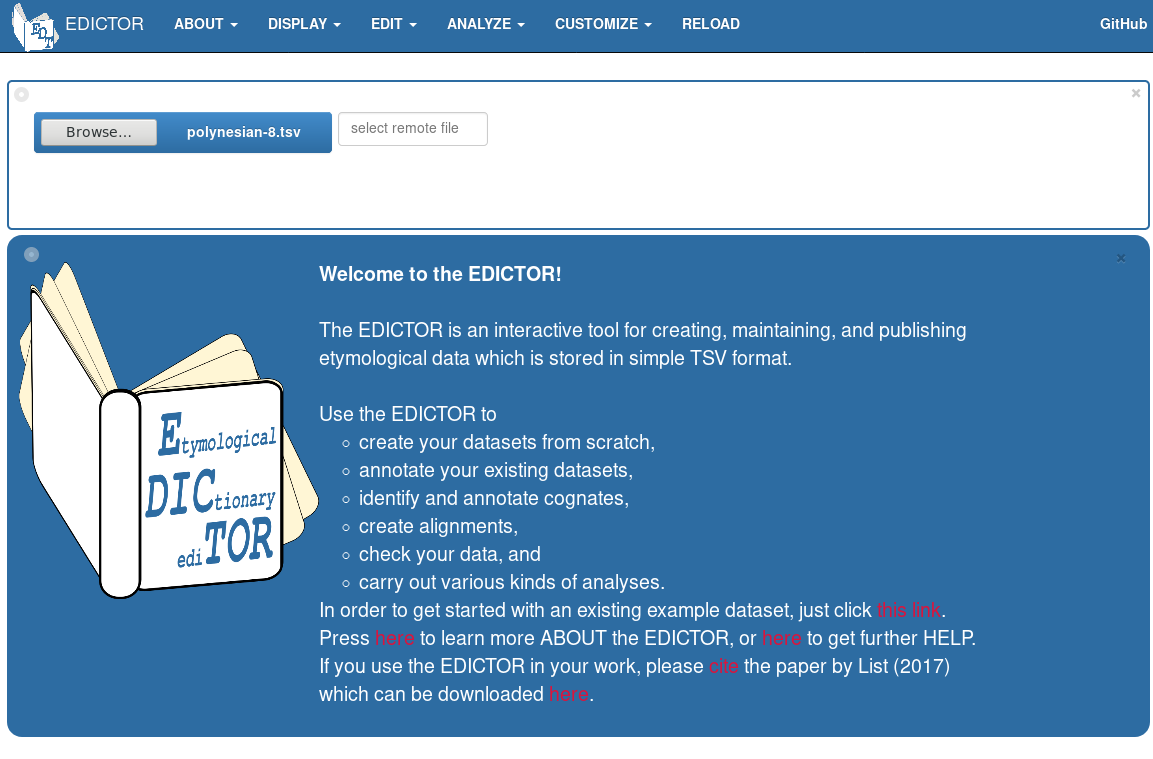
\includegraphics{images/figure-1.png}
\caption{Welcome page of the EDICTOR.}
\end{figure}

Since the EDICTOR is written in plain JavaScript, no data will be send
to the server, but all data will stay on the computer of the user alone.
Thus, essentially no data is uploaded somewhere else. Linguists are
sometimes afraid that their data might be stolen by their colleagues.
Apart from the fact that this is unlikely, given that everybody will
know where the original data came from, and that not many linguists
would papers on languages where they do not know the sources, and where
they do not know on what judgments the cognate assignments were based,
not to speak of the fact that normally, the data people work on does not
list all the sources, users of the EDICTOR should know that although the
BROWSE procedure by which they can load their data looks like an upload
button in other software applications, no upload is carried out. Data
will rest on the client computer and not leave it during the whole time
the EDICTOR is being used.

Once you have browsed your file, a red window will open, showing that
the file was successfully loaded:

\begin{figure}
\centering
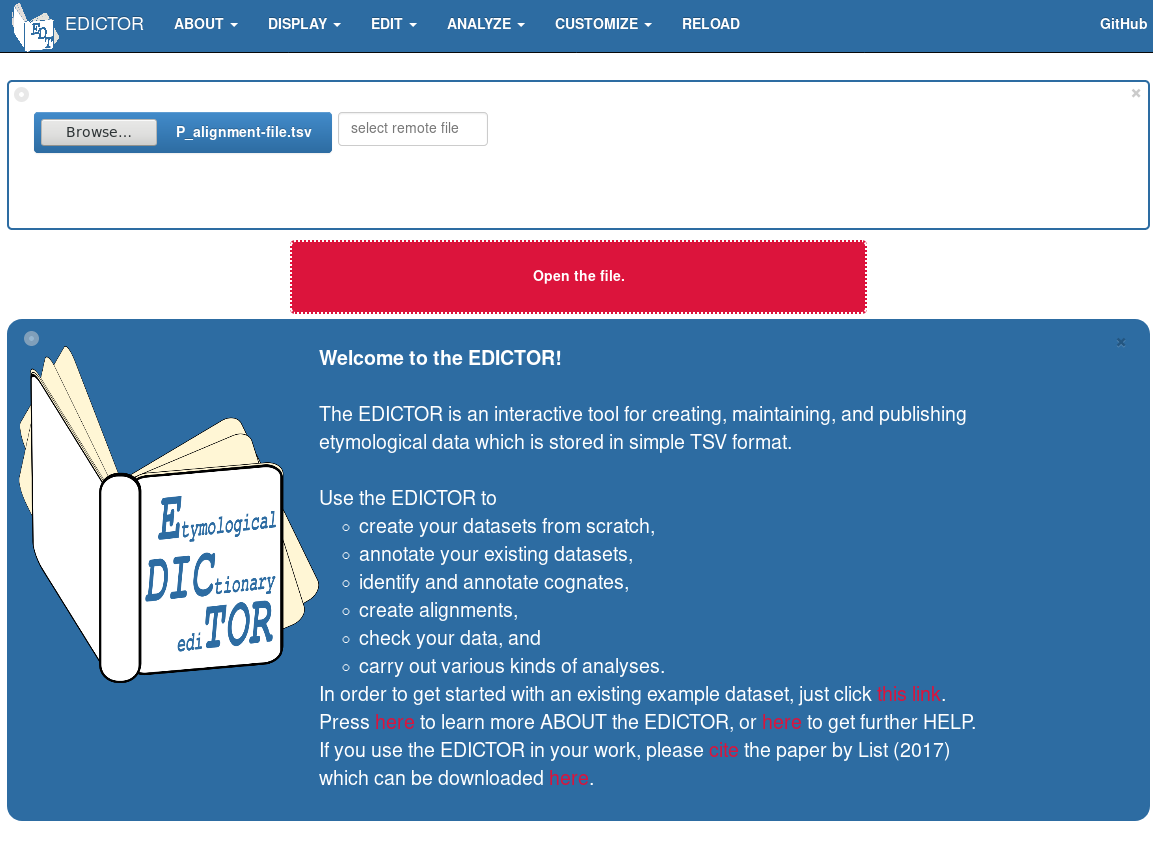
\includegraphics{images/figure-2.png}
\caption{Loading data with EDICTOR.}
\end{figure}

By clicking on the red field, you initiate your EDICTOR session, and the
Wordlist panel will pop up.

\begin{figure}
\centering
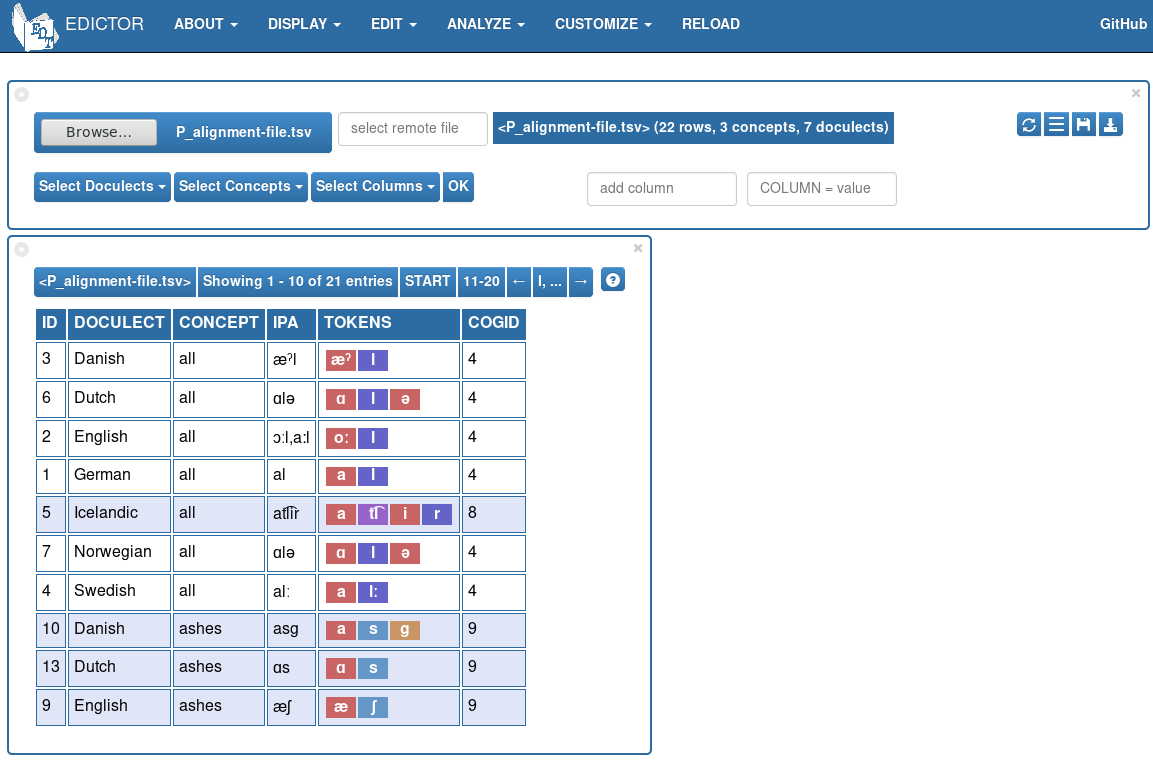
\includegraphics{images/figure-3.png}
\caption{Wordlist panel in EDICTOR.}
\end{figure}

As you can see from the figure, the data that we just created in the
previous section is now rendered through the EDICTOR. In the top panel,
the Menu panel, basic statistics about the file is displayed (i.e., that
it contains 22 rows, 7 languages, and 3 concepts). On the top-right of
the Menu panel, you can see four different buttons:

\begin{figure}
\centering

\includegraphics{images/figure-4.png}
\caption{Buttons for refreshing, saving, and loading files.}
\end{figure}

If you hover over the buttons with your mouse, information on their
function will be displayed. The first button serves to refresh the data.
If you have the impression that the EDICTOR is not doing the right
thing, it may be useful to press this button to make sure all data is
correctly analysed. The second button will switch of the three basic
Filters provided by the Menu panel (see below for more details on the
filters). The third and fourth button are essential to export the data
after you have edited them. In general, the first button stores the data
internally in your webbrowser and does not save them forever (especially
if you have rigid privacy options that delete cookies and internal
storage after closing your webbrowser). The fourth button will
``download'' the data, i.e., it will export them in text-form and
usually store them in your ``Download'' folder of your system. When
working with the EDICTOR, I recommend to press both buttons regularly
all 10 minutes to make sure no data is lost. This can be conveniently
done with help of the shortcuts \texttt{\textless{}CRTL\textgreater{}S}
and \texttt{\textless{}CTRL\textgreater{}E}. When re-entering an EDICTOR
session, all you have to do is then to load the file you last edited
into the system, and you can keep on working where you ended.

This is further enhanced by the fact that the EDICTOR will remember
certain operations and write them to the text-files. For example, when
you selected only one concept with help of the Filter options in the
Menu panel and then export your file, the EDICTOR will remember this and
upon re-import it will only render those concepts which you selected.
You can test this behaviour by taking the file
\texttt{P\_alignment-file-edited.tsv} and importing it into the EDICTOR.
You will see that it only displays the first concept (``I'') if you use
this file, but all concepts if you use the
\texttt{P\_alignment-file.tsv}.

\begin{figure}
\centering
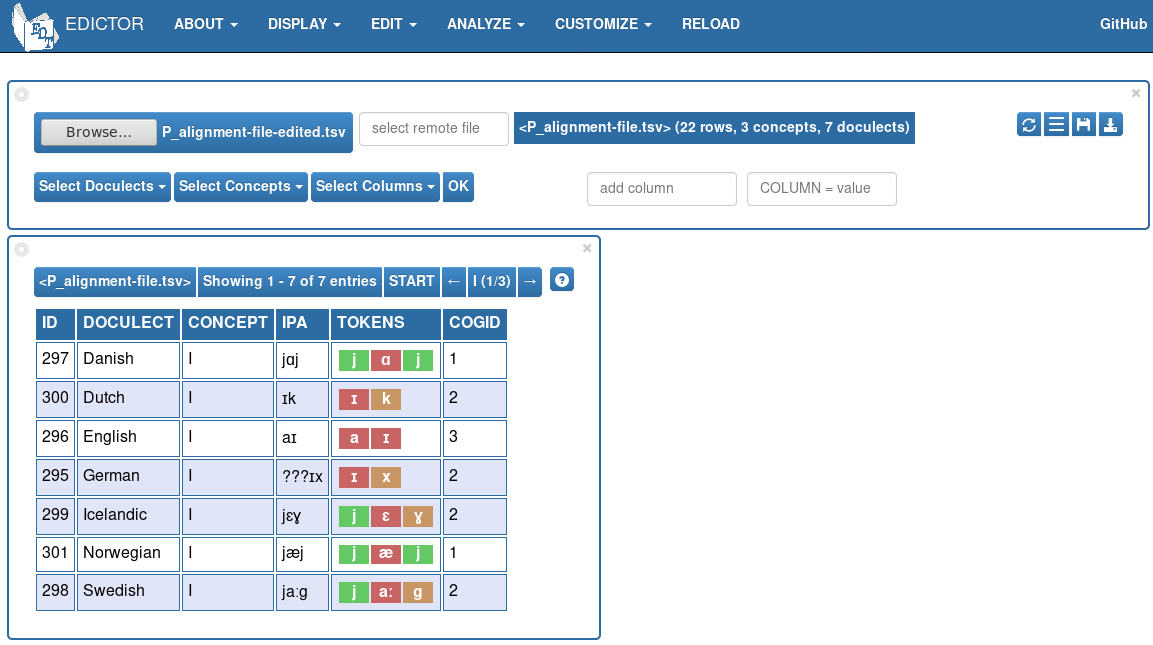
\includegraphics{images/figure-5.png}
\caption{Loading options along with the file in EDICTOR.}
\end{figure}

Each panel has a little circle symbol on its top left. By clicking on
this symbol, you can drag the panel and arrange them to your needs. Each
panel can further be switched off by clicking on the cross in the
top-right. In order to switch a panel back on, you need to go to the
menu in the very top of the EDICTOR and click on the respective panel.
Most panels also offer quick help. In order to view it, press on the
top-right button with the question-mark. Press on it again to display
the panel instead of the help message.

If you click in the top-level menu on DISPLAY-\textgreater{}SETTINGS, a
new window will open which allows you to modify or set certain options.

\begin{figure}
\centering
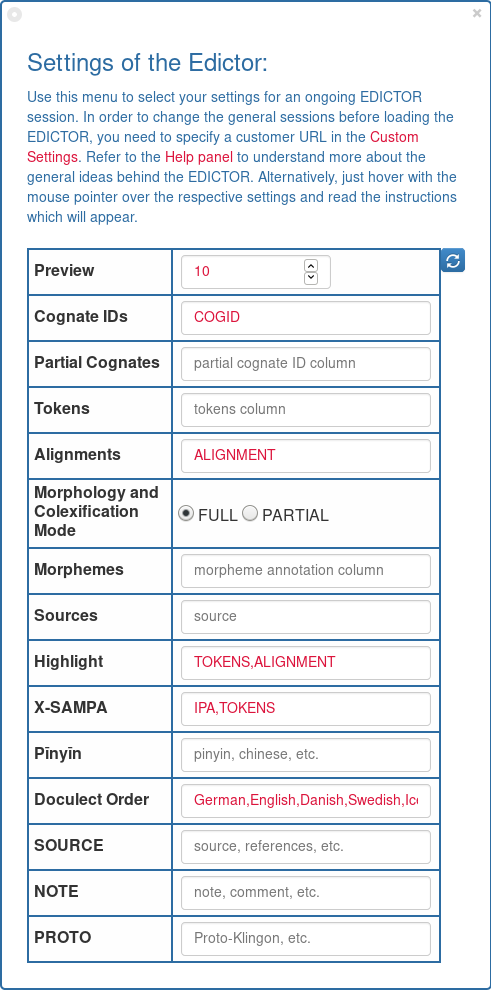
\includegraphics{images/figure-6.png}
\caption{Settings panel in the EDICTOR.}
\end{figure}

By hovering with the mouse over the optionso on the left of this menu,
more information on the different functions of these options will be
shown. What is crucial for cognate annotation is to tell the EDICTOR in
which column your cognate sets are stored, and in which column your
alignments can be found. Usually the EDICTOR guesses independently, but
you can likewise specify your own preferred column for cognate sets or
alignments.

The EDICTOR will also ``highlight'' certain values, i.e., render them
differently than they appear in your original data, as you can see when
looking at the TOKENS column. To change this behaviour, you can modify
the values for the Highlight option. Similarly, if you do not want that
the data you type is automatically treated as X-SAMPA input, you should
empty the values in the X-SAMPA option. Having modified your preferred
options, you should press on the REFRESH button on the top-right of the
Settings panel.

\subsection*{3.3 Hands on the Data: The Wordlist
Panel}\label{hands-on-the-data-the-wordlist-panel}
\addcontentsline{toc}{subsection}{3.3 Hands on the Data: The Wordlist
Panel}

The Wordlist is the central view of the EDICTOR and all other ways to
inspect and edit the data are centered around the Wordlist panel. If you
open a file the first time, you may be surprised that you see only 10
items. This is the default preview of your data. For a quick browsing of
the data, you can click on the buttons to the left and the right of the
START symbol on top of the Wordlist panel. If you just loaded your data,
there won't be a browse-button on the left of START, but only on the
right, indicating the next number of items which you can inspect. In
this way, you can go forward and backward through your data. You can
conveniently scroll through the data with help of the page-up and
page-down keys on your keyboard. If you prefer a larger preview, you can
change this in the Settings. As a new feature, we currently test a new
way to browse the wordlist data on a concept-per-concept basis. In order
to do so, just click on the arrows in the top menu of the Wordlist
panel.

\subsubsection*{Editing Data}\label{editing-data}
\addcontentsline{toc}{subsubsection}{Editing Data}

A general feature of the Wordlist panel is to offer a quick way to edit
the data. Essentially, each cell in the Wordlist can be edited by
clicking one time on the cell and modifying the entry. In order to save
the data, you need to press either the ENTER key, or one of the UP and
DOWN keys, which will automatically bring you to the next cell above or
beyond the cell you just edited.

Instead of editing the data, you can also use the keys to navigate
quickly through your data. While UP and DOWN key work as expected, you
need to press CTRL in addition to ``LEFT'' and ``RIGHT'' to jump from
one cell to the cell at the left or the cell at the right. This is
important, since otherwise you would have difficulties in editing the
content of a cell, where LEFT and RIGHT are also needed to navigate.

\subsubsection*{Interaction between
Columns}\label{interaction-between-columns}
\addcontentsline{toc}{subsubsection}{Interaction between Columns}

One of the most crucial features of the EDICTOR is the interaction
between different columns in your data. As a general rule, if a cognate
set identifier is found in your data (default \texttt{COGID}),
right-clicking in a cell with your mouse will open an alignment window
in which you can align the data by simply clicking on it (see below).
Right-clicking on other columns will store the data in cache.
Right-clicking again will insert the stored value in the field on which
you clicked.

\subsubsection*{Adding and Deleting
Rows}\label{adding-and-deleting-rows}
\addcontentsline{toc}{subsubsection}{Adding and Deleting Rows}

If you want to add a new row to your data or delete an existing row, you
can click on the values in the ID column. This will open a dialog from
which you can select your options.

\subsubsection*{Filters}\label{filters}
\addcontentsline{toc}{subsubsection}{Filters}

A crucial and important function for convenient data-editing are the
filters provided by the Menu panel. Three filters are offered here, plus
one largely experimental filter based on string comparison.

\begin{figure}
\centering

\includegraphics{images/figure-7.png}
\caption{Filters for the Wordlist panel of the EDICTOR.}
\end{figure}

When applying a filter, you first carry out your selection by pressing
on the respective buttons, and then need to press on the OK button on
the right of the three main filters to submit the changes. To use the
column-filter on the right of the filter menu, write your filter-query
in the form \texttt{column=value} exclude all rows in which the column
you selected does NOT contain the string, or write
\texttt{column==value} to filter only those rows which have the exact
same string as content. Thus, to filter, for example, all cognate sets
which contain a 1, you could write \texttt{cogid=1}. In order to filter
all cognate sets which are identical with 1, you should write
\texttt{cogid==1} and then press enter (note that both capital and
lowercase spelling are supported).

\subsubsection*{Sorting}\label{sorting}
\addcontentsline{toc}{subsubsection}{Sorting}

By double-clicking on a given column (apart from the ID column), the
data will be automatically sorted. Double-clicking again will sort the
data in the opposite direction, double clicking a third time will
restore the original order.

\subsection*{3.4 Finding Cognates: The Cognate Sets
Panel}\label{finding-cognates-the-cognate-sets-panel}
\addcontentsline{toc}{subsection}{3.4 Finding Cognates: The Cognate Sets
Panel}

In order to offer an efficient and convenient way to identify cognate
sets, the EDICTOR offers the Cognate Sets panel. This panel can be
opened by clicking on EDIT in the main menu and then on Cognate Sets. It
will open a new window in which, starting from the first concept in your
data, all languages are listed in tabular form along with their
alignments and cognate sets.

\begin{figure}
\centering
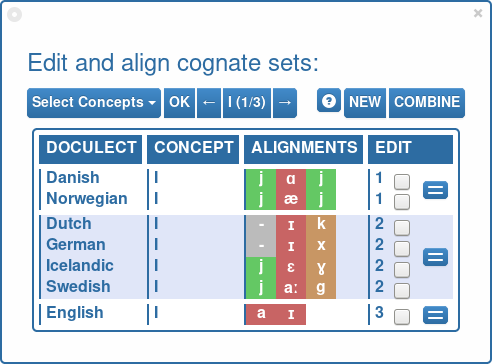
\includegraphics[width=0.5\textwidth]{images/figure-8.png}
\caption{Cognate Sets panel of the EDICTOR.}
\end{figure}

You can select concepts by using the filter on the top left (which also
allows you to select more than one concept), or by clicking on the
arrows to quickly navigate from one concept to the other. As a general
rule, pressing the OK button will refresh your data, which is important
when you carry out alignment analyses, as they will not be automatically
refreshed after they were submitted.

\subsubsection*{Cognate Set Annotation}\label{cognate-set-annotation}
\addcontentsline{toc}{subsubsection}{Cognate Set Annotation}

There are two basic operations that are supposed to help in editing
cognate sets. One is called \emph{new} and one is called \emph{combine}.
For each of the two procedures you need to select words by clicking on
the selection fields on the right of the cognate sets table. By clicking
on \emph{new} you will create new cognate identifiers for the respective
words. By clicking on combine, all cognate sets with the same cognate
identifier as the ones you identified by clicking on them will be merged
to form a large new group which retrieves the smallest of the cognate
identifiers in the cluster.

Hence, if you press on one representative of each of the three cognate
sets shown in the previous figure, and then on combine, it will merge
all cognate sets into one class, automatically selecting the lowest
value for the cognate ID.

\begin{figure}
\centering
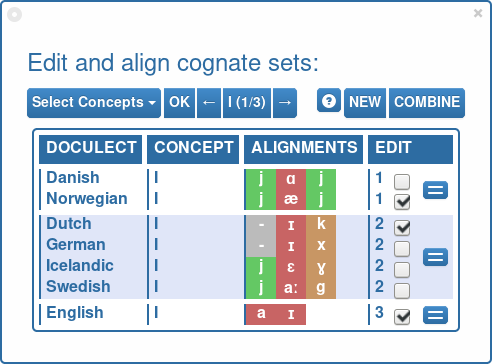
\includegraphics[width=0.5\textwidth]{images/figure-9.png}
\caption{Annotation of cognate sets.}
\end{figure}

\subsubsection*{Alignment of Cognate
Sets}\label{alignment-of-cognate-sets}
\addcontentsline{toc}{subsubsection}{Alignment of Cognate Sets}

Having assigned your words to cognate sets, you should align your data.
This can be conveniently done by clicking on the alignment symbol next
to each cognate set in the EDIT field. If you press this button, a
window will pop up, offering different options for the alignment
analysis.

\begin{figure}
\centering
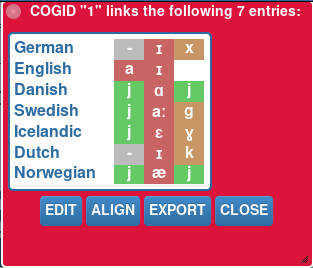
\includegraphics[width=0.5\textwidth]{images/figure-10.png}
\caption{Alignment of cognate sets.}
\end{figure}

If you press on EDIT, you will enter the EDIT mode where you can push
the sequences around by clicking on sounds or gaps. As a rule, if you
click on a sound, this will insert a gap to the left of the sound. If
you click on a gap, the gap will disappear. In order to drag a sound to
the left, click on the arrow-symbol on the left of the sequence. If you
want to push and pull more than one sequence at the same time, you can
click on the language names in the left. This will mark them as being
linked, and when you now click on any of those sequences, gaps will be
inserted or deleted in all sequences assigned to the same group.

\begin{figure}
\centering
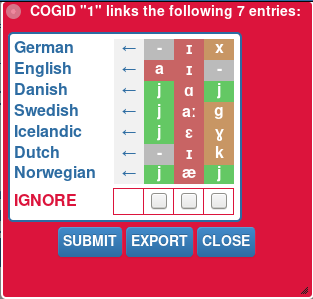
\includegraphics[width=0.5\textwidth]{images/figure-11.png}
\caption{Editing alignments.}
\end{figure}

By clicking into the IGNORE row on the bottom of the alignment, you may
mark parts of your alignment as irrelevant for your investigation. This
may come in handy when you work with words where you can only identify
common roots, while the morphology largely differs. It is also a
convenient short-cut when working with compound words and high amounts
of partial cognates, although we recommend to use the more powerful
Partial Cognate Set panel for this kind of analysis.

As a final feature, you can have the EDICTOR align the data
automatically, although the results may be disappointing. The algorithm
used for this purpose is a very simple one that only takes the longest
string and aligns all other strings to it. Nevertheless, especially when
dealing with larger alignments, it may come in handy.

\subsubsection*{Integration of Wordlist and Cognate Set
Panel}\label{integration-of-wordlist-and-cognate-set-panel}
\addcontentsline{toc}{subsubsection}{Integration of Wordlist and Cognate
Set Panel}

If you leave the Wordlist panel open while annotating your cognate sets,
you will see that the Wordlist panel will change content when you switch
to the next concept. In fact, it will always display the same concepts
which you have selected in the Cognate Sets panel. Similarly, when using
the concept-navigation in the Wordlist panel, the cognate sets will be
synchronized accordingly. This makes it very convenient to edit the data
at the same time when carrying out the cognate judgments. For example,
if you realize that an entry is wrongly segmented, you may just change
it quickly in the Wordlist panel and then go on and align it again. The
integration across panels is one of the crucial features of the EDICTOR
and you will see, when exploring the tool further, that this interaction
holds for many of the different panels.

As a further important point that facilitates working with cognate sets
in the Wordlist panel is the fact that inserting any non-numeric
character into the column which stores the cognate sets for a given
analysis will automatically search for the next free identifier which
has not yet been used. This prevents errors from assigning the same
number multiple times and illustrates the usefulness of using specific
interfaces rather than ad-hoc formats when preparing data in historical
language comparison.

\subsection*{3.5 Enhanced Cognate Annotation: The Partial Cognate Sets
Panel}\label{enhanced-cognate-annotation-the-partial-cognate-sets-panel}
\addcontentsline{toc}{subsection}{3.5 Enhanced Cognate Annotation: The
Partial Cognate Sets Panel}

With a few exceptions (\href{:ref:Starostin2013}{Starostin 2013:
119-123}), \emph{partial cognacy}
(\href{http://bibliography.lingpy.org?key=Trask2000}{Trask 2000:248}),
resulting from morphological processes such as derivation and
compounding, has long been disregarded as a problem for phylogenetic
reconstruction. Only recently more and more evidence has been assembled
to show that it may even crucially impact on the results of phylogenetic
reconstruction (List 2016,
\href{http://bibliography.lingpy.org?key=Hill2017a}{Hill and List
2017}). Even if partial cognates are rare in a given dataset, it is
useful to think of ways how to handle them consistently. While the
Cognate Sets panel of the EDICTOR allows for quite some flexibility in
assigning words to cognate sets, and especially the possibility to mark
those parts which are relevant for a cognate set in the alignment, it
may reach its limits if the amount of partial overlap in cognate words
is large.

For this reason, the EDICTOR offers an explicit way to annotate partial
cognates which is theoretically largely superior to binary cognate
coding in so far as it allows to assign only parts of words to different
cognate sets. The disadvantage is that unless the data can be obviously
segmented into morphemes, as in the case of many SEA languages, users
will have to do this manually. On the other hand, given that linguists
who seek to reconstruct a language families history usually demand the
highest level of expertise anyway, it seems that there is no serious way
around the problem of segmenting the data morphologically, even if one
only splits off the root from the rest.

As mentioned before, morphological segmentation can be carried out by
splitting the TOKENS with help of the plus-character (\texttt{+}) or the
underscore (\texttt{\_}). Although both characters may have a different
meaning for linguists, they are not further distinguished when it comes
to annotating partial cognates.

\subsubsection*{Preliminaries for Partial Cognate
Identification}\label{preliminaries-for-partial-cognate-identification}
\addcontentsline{toc}{subsubsection}{Preliminaries for Partial Cognate
Identification}

In order to annotate partial cognates with the EDICTOR, your need to
specify the column in which you want to store partial cognate sets. In
fact, even if your data is not morphologically segmented, you can just
specify a column and annotated your data with help of the Partial
Cognate Sets panel, and you may even think that it is even more
intuitive and convenient to use than the classical Cognate Sets panel,
given its improved operations. However, if you face problems in
identifying cognates consistently in your data or aligning your words,
you should definitely go through the pain of annotating your data for
morpheme boundaries and assigning cognate sets on the basis of partial
cognates.

The default name for partial cognate sets is \texttt{COGIDS}. If you
prepared a file in which you add such a column, you can immediately use
the Partial Cognate Sets panel. If this is not the case, you will have
to specify your column in the Settings panel. To allow you to test this
behaviour, we prepared a test-file, called \texttt{E\_chinese.tsv},
which provides partial cognates and pre-segmented data for six Chinese
dialects (prepared by Yunfan Lai and Johann-Mattis List as part of the
CALC project).

If you open the panel, a window similar to the Cognate Sets window will
pop up, with the difference being that cognate identifiers are now given
in additional columns, with one empty column each time, showing you the
next cognate identifier to which you can assign new data.

\begin{figure}
\centering
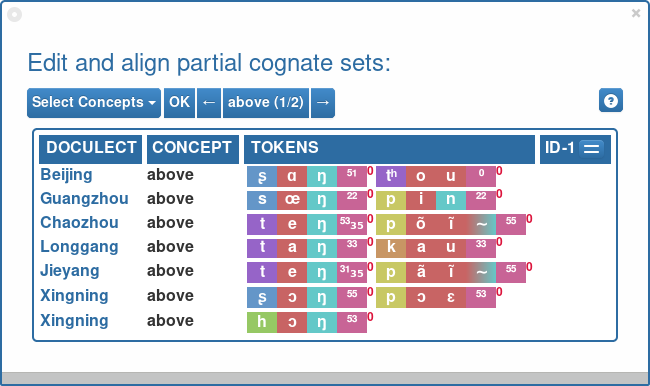
\includegraphics[width=0.8\textwidth]{images/figure-12.png}
\caption{Partial Cognate Sets in the EDICTOR.}
\end{figure}

If no cognate sets have been distributed so far, all the morphological
segments in your data will be given a little 0 in red to their top
right. You can now select morphemes across the languages by clicking on
them. Once you have done this, you can click on the next free ID on the
right to assign the morphemes to this cognate set. If you want to refine
an analysis, you can delete an item from a given cognate set by clicking
on it inside the column with the cognate identifiers.

\begin{figure}
\centering
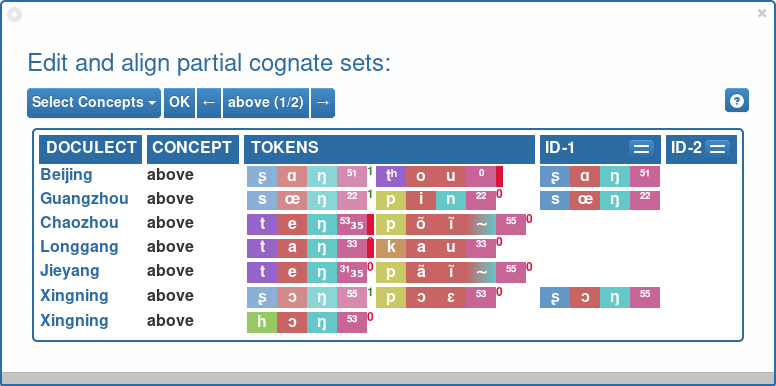
\includegraphics{images/figure-13.png}
\caption{Editing partial cognate sets.}
\end{figure}

You can also align the data, simply by clicking on the alignment button,
and you can likewise sort the data in various ways, by rightclicking on
a given column with a cognate set identifier. If you have a look at the
Wordlist panel after assigning cognate identifiers, you will see that
the COGIDS column will regularly contain as many numbers, separated by a
space, as there are morphemes per word. The numeric annotation thus
follows the order of morphemes in the base form of the word and provides
a unique identifier similar to the cognate set identifiers used by
EDICTOR for full cognates.

\begin{figure}
\centering
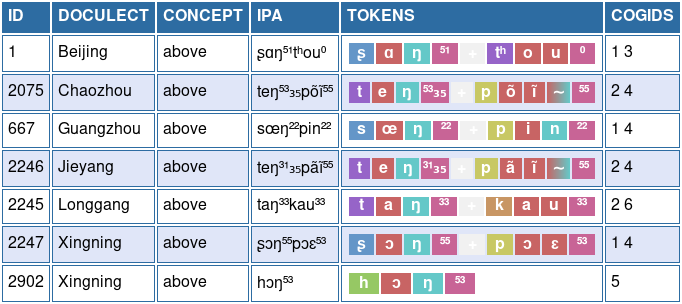
\includegraphics{images/figure-14.png}
\caption{Representation of partial cognates in the Wordlist
panel.}
\end{figure}

\section*{4 Analysing Data with
EDICTOR}\label{analysing-data-with-edictor}
\addcontentsline{toc}{section}{4 Analysing Data with EDICTOR}

In addition to allowing for a consistent annotation of linguistic data
for the purpose of historical language comparison, the EDICTOR also
offers different ways to analyze the data. These procedures and methods
are summarized under the ANALYZE header in the main menu of the EDICTOR.
Using these additional features may require additional columns in your
file, as you will see in the following.

\subsection*{4.1 Inspecting Sounds and Transcriptions: The Phonology
Panel}\label{inspecting-sounds-and-transcriptions-the-phonology-panel}
\addcontentsline{toc}{subsection}{4.1 Inspecting Sounds and
Transcriptions: The Phonology Panel}

Let us quickly start by exploring the Phonology panel. When loading our
sample file \texttt{E\_chinese.tsv} and clicking on
ANALYZE-\textgreater{}Phonology, a new panel will open that allows you
to select one of the doculects. Let us choose Beijing Chinese, as the
phonology is farely well understood. The panel will now list all of the
sounds encountered in the TOKENS column for Beijing Chinese:

\begin{figure}
\centering
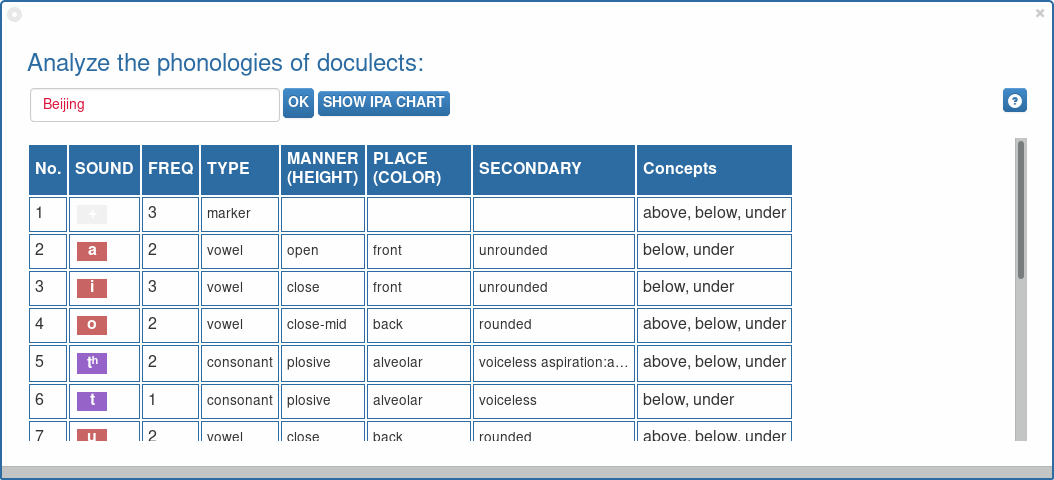
\includegraphics{images/figure-15.png}
\caption{Phonology inspection with the EDICTOR.}
\end{figure}

By double-clicking on the different headers, you can sort the data
accordingly. The columns list apart from the sound itself and its
frequency of occurrence also some basic features (as far as the sounds
are known to EDICTOR, which is again a reason why one should try to use
the standards that are underlying the tool). The column on the right is
called Concepts and it shows all the concepts in which the sound occurs.
If you click on the cell with the concepts, the Wordlist panel will be
automatically filtered, showing only those concepts for Beijing Chinese
where the sound occurs. This is convenient for checking erroneous sounds
in your data. By clicking on the button SHOW IPA CHART, you can see an
IPA chart which assembles all sounds which can be identified in the
relevant cells. Sounds which cannot be identified will be listed in
isolation. In our sample, we don't have many words, so it is not
entirely fun or enlightening to review the sounds, but in general, the
IPA chart is useful to detect missing spots in regular series, be it due
to sparse data or gaps in the phonological system.

\subsection*{4.2 Enhanced Morphological Annotation: The Morphemes
Panel}\label{enhanced-morphological-annotation-the-morphemes-panel}
\addcontentsline{toc}{subsection}{4.2 Enhanced Morphological Annotation:
The Morphemes Panel}

We have mentioned partial cognates before, especially pointing to the
importance of using this way of cognate annotation if the morphology of
your languages is complex. An additional way to account for complex
morphology is to use the Morphology panel to analyze full and partial
colexifications in your data. This is extremely useful to detect
dependencies of your cognate sets resulting from underspecification as
in languages which have the same word for ``arm'' and ``hand'', but also
to assign language-internal cognates.

\subsubsection{Basic Inspection of Partial
Colexifications}\label{basic-inspection-of-partial-colexifications}

In order to carry out this kind of analysis, you will need a column
called MORPHEMES (which is detected and assigned as such by default) or
you will have to assign one of your columns to this group manually by
using the Settings panel. In our case, we use the column MORPHEMES,
which we already added to the file \texttt{E\_chinese.tsv}. When
clicking on ANALYZE-\textgreater{}Morphology, a new panel will open and
you can again specify a language variety. We will again use Beijing
Chinese for this purpose. Make sure to select PARTIAL as MODE of
inspection, and leave the other items at the default provided by the
tool. The resulting analysis will look as follows:

\begin{figure}
\centering
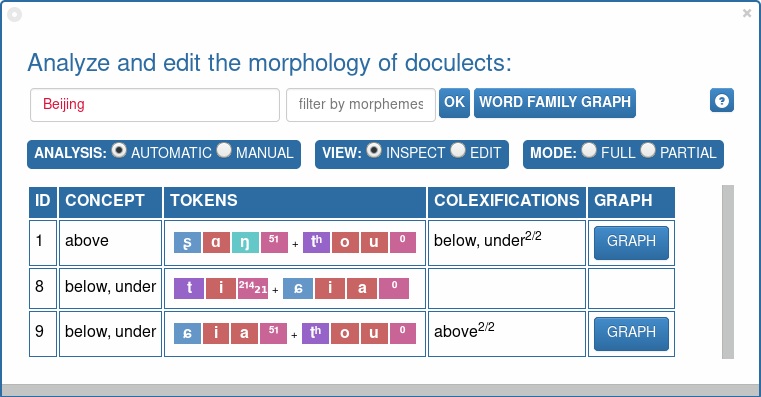
\includegraphics[width=0.8\textwidth]{images/figure-16.png}
\caption{Enhanced morphology inspection with the EDICTOR.}
\end{figure}

The information with which you are provided here can be read as follows:
The entry ``above'' in Beijing Chinese is partially colexified with the
entry ``below, under''. The superscript numbers divided by a slahs after
the entry in the COLEXIFICATIONS cell indicate that we are talking about
the second element of ``above'' and the second elemnt of ``below,
under''. If you click on the GRAPH button, a pop-up window will open and
visualize the structure:

\begin{figure}
\centering
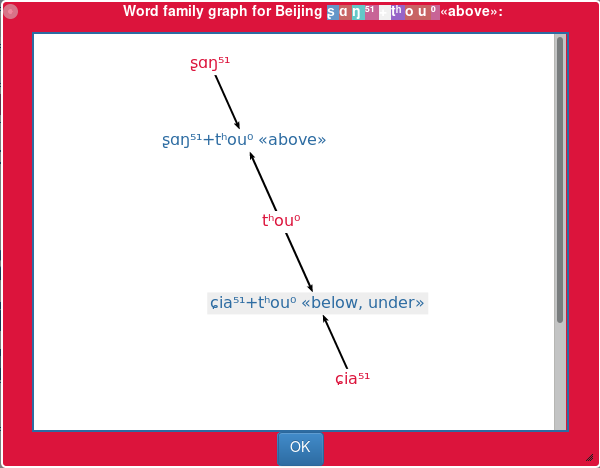
\includegraphics[width=8cm]{images/figure-17.png}
\caption{Graph representation of morphological relations.}
\end{figure}

This is bipartite graph constructed from shared elements in the data
(see \href{http://bibliography.lingpy.org?key=Hill2017a}{Hill and List
2017}) for details on this datastructure.

\subsubsection{User-Annotated Partial
Colexifications}\label{user-annotated-partial-colexifications}

An additional and more powerful way to not only analyze but also
annotated your data is to provide your judgments on language-internal
cognacy. In our data for the Chinese dialects, suffixes as well as root
elements of the counterparts of ``above'' and ``below, under'' are
recurring. In Beijing Chinese, for example,
\texttt{{[}}tʰou⁰\texttt{{]}} is a frequently recurring suffix, which
formerly meant ``head''. In the word for ``above''
\texttt{{[}}ʂɑŋ⁵¹tʰou⁰\texttt{{]}}, the first element usually functions
as a noun, but it could be labeles as bearing the main meaning
``above''. We could thus characterize the word as ``above'' + ``head'',
and if we insert these values, separated by a space into the MORPHEMES
cell of the word, it will be rendered in a specific form that indicates
the specific meaning of the elements of the word. The sample data has
been annotated for all languages in this way, as you can see when
selecting the column MORPHEMES in the major filter sections of the
Wordlist panel as shown in Figure 18.

\begin{figure}
\centering
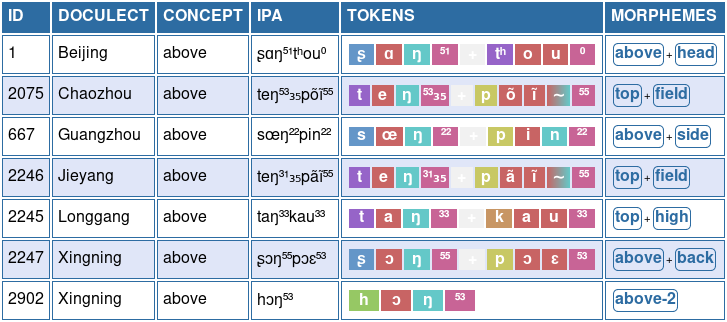
\includegraphics{images/figure-18.png}
\caption{User-annotation of partial colexifications and
language-internal cognates.}
\end{figure}

As an additional important feature which helps to make binary cognate
decisions for partial cognates more transparent, you can right-click on
a given morpheme in the morpheme panel in order to indicate that it does
not contribute to the overall cognate decision you make. If you do so,
the labels in the MORPHEME column will be internally prefixed by an
underscore. In the Wordlist panel, this will be rendered by decreasing
the font-size of the relevant morpheme while at the same time increasing
its transparency. As a result, you can easily spot which elements share
the main morpheme in your data, as shown in Figure 19.

\begin{figure}
\centering
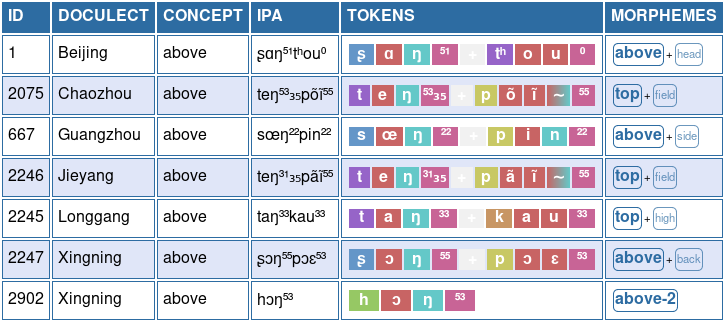
\includegraphics{images/figure-19.png}
\caption{Inspecting user-annotation of morphological
structure.}
\end{figure}

\subsubsection{Browsing User-Annotated Partial
Colexifications}\label{browsing-user-annotated-partial-colexifications}

You can also browse your user-annotated partial colexifications in the
Morphology panel. In order to do so, just set the radio button in
ANALYSIS to MANUAL and click on OK. The resulting table combines the
information in the TOKENS and the MORPHOLOGY column, which makes it
convenient to inspect the morpheme structure of the compounds as shown in Figure 20.

\begin{figure}
\centering
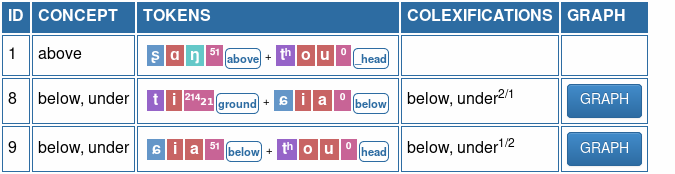
\includegraphics{images/figure-20.png}
\caption{Browsing user-annotation and partial
colexifications.}
\end{figure}

If you now set the radio button in VIEW from INSPECT to EDIT and click
again on OK, you can edit the morphemes by clicking into the MORPHEMES
cell without editing the data in the Wordlist panel. This will prove
useful if you are working on language families whose morphology you do
not yet fully understand. As a general rule, the algorithms underlying
EDICTOR will identify all morphemes which you assign the same string
(without spaces, so use an underscore or a dash, if you want to annotate
longer phrases) as being judged to be cognate \emph{inside} the given
language. This principle will also prove extremely useful if you try to
identify cognates across different meanings, as polysemy is the first
step to identify cognates across meaning classes.

\subsection*{4.3 Analysing Cognate Sets: The Cognate Sets
Panel}\label{analysing-cognate-sets-the-cognate-sets-panel}
\addcontentsline{toc}{subsection}{4.3 Analysing Cognate Sets: The
Cognate Sets Panel}

If you assign words to cognate sets, it is useful to check the overall
patterning of the cognate sets in your data. In order to do so, make
sure that you have selected \emph{all} concepts in your data, using the
concepts filter, and then click on ANALYZE-\textgreater{}Cognate Sets. A
pop-up window will open and ask whether you want to inspect full
cognates or partial cognates. As we have already assigned our Chinese
words to full cognate sets, following our principle of user-defined
salience of morphemes in words briefly mentioned above, we select
``full'' for this test. In order to render the analysis more
interesting, however, we will first delete the words in Xingning Chinese
for the concept ``above'' by clicking on the ID field and selecting
``delete row''. If we now click on OK, a table will appear that shows
all the cognate sets in the data, as shown in Figure 21.

\begin{figure}
\centering
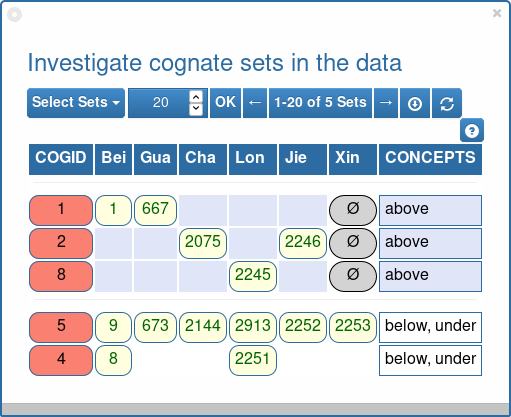
\includegraphics[width=0.6\textwidth]{images/figure-21.png}
\caption{Analyzing cognate sets.}
\end{figure}

This table shows the cognate sets in the first row (clicking on them
will open the alignemnt view), and the words (represented by their
unique IDs) in each cell in which a language has a valid reflex. Missing
data is represented as shown for Xingning Chinese for the concept
``above'', which we deleted before, namely in gray background with a the
Ø symbol, which serves to indicate gaps in the EDICTOR. When clicking on
the entries in the table, you can view the word underlying the cognate
set. By clicking on the export-button, you can even save the data in
Nexus-format, as shown below:

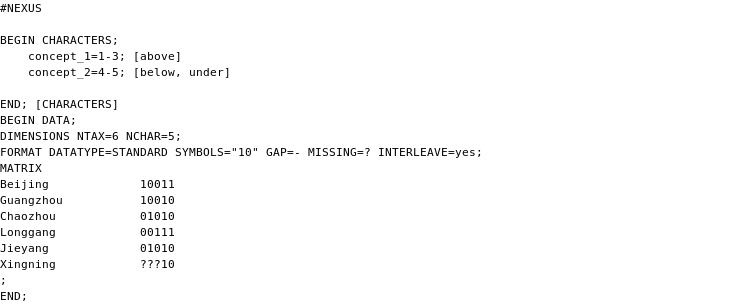
\includegraphics[width=\textwidth]{images/code-nexus.png}

This text file can be directly be used with software packages such as
SplitsTree to create splits networks of distance-based trees. It
illustrates another advantage of properly preparing your data with help
of software tools: while you may have an extremely hard time in trying
to convert your data in Nexus format when doing it manually, the EDICTOR
just provides you with the export for free.

\subsection*{4.4 Analysing Sound Correspondences: The Correspondences
Panel}\label{analysing-sound-correspondences-the-correspondences-panel}
\addcontentsline{toc}{subsection}{4.4 Analysing Sound Correspondences:
The Correspondences Panel}

As a last illustration of the multitude of possibilities which the
EDICTOR offers for consistent data annotation and inspection, let us
have a look at the sound correspondences in our data. Here the EDICTOR
applies a new method which was developed in close collaboration with
Nathan W. Hill (for an early account
\href{http://bibliography.lingpy.org?key=List2017TALKk}{List and Hill
2017}) and is currently being finalized. This new method allows to
inspect the correspondence patterns in the alignments of the data by
clustering all alignment sites into compatible correspondence sets,
thereby automatically checking the regularity of a given alignment site
and therefore also the regularity of a given cognante set. This panel,
the Correspondences panel, uses a rough approximate solution for the
problem of identifying correspondence patterns, which would be otherwise
too expensive to be applied from within JavaScript software running in
the browser.

For our illustration, we use the file \texttt{E\_germanic.tsv} which
takes cognate judgments as provided by the Tower of Babel project for a
sample of 7 Germanic varieties along with phonetic transcriptions added
by \href{http://bibliography.lingpy.org?key=List2014d}{List (2014)}. For
this experiment, the data was further automatically aligned with help of
LingPy. When loading this file into the EDICTOR and opening the
Correspondence Patterns panel via ANALYZE-\textgreater{}Correspondence
Patterns, a window will open and asking for the underlying mode (partial
of full cognacy). For the Germanic data, we assume full cognacy, which
means we can click the OK button directly. The resulting table which
opens shows all correspondence patterns observed in the data and
automatically clusters them into groups of compatible sites. Note that
the algorithm is not accurate, but comes very close to a good result.
Better analyses with LingPy are currently in preparation. By adjusting
the PREVIEW, we can define how many correspondence patterns we want to
watch at the same time. You can further select specific sounds by using
the filter provided on the left of the menu above the table. The sounds
selected are automatically those sounds of the first language in the
sample, which is German in our case. If you have proto-languages in your
data, you can select one of them via the Settings panel, and it will be
displayed as the first language in this analysis. For our purpose, we
filter all instances of \texttt{{[}}t͡s\texttt{{]}} in German (they are
scattered over the data, as they occur in 6 distinct patterns which are
not compatible with each other.

\begin{figure}
\centering
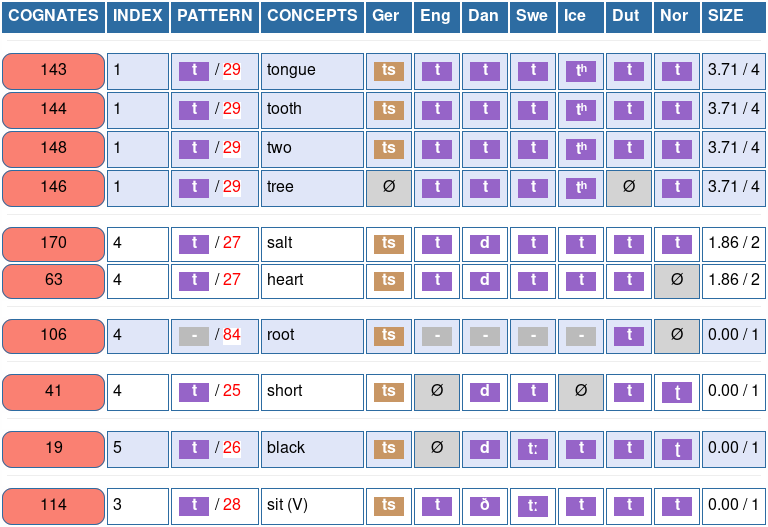
\includegraphics{images/figure-22.png}
\caption{Analyzing correspondence patterns.}
\end{figure}

As we can see from this view, we get an immediate impression regarding
the amount of different patterns in the data in which German shows a
\texttt{{[}}t͡s\texttt{{]}}. As a matter of fact, all these patterns go
back to the same proto-sound, but the environments which trigger changes
in the daughter languages are all different. Swedish, for example, shows
a retroflex in the word for ``black'' due to the fact that it is
preceded by an \texttt{{[}}r\texttt{{]}}. The words for ``root'' are
swapped in some languages, and ``salt'' and ``heart'' have the
Proto-Germanic \texttt{*}\emph{t} in final position instead of the
initial position. In fact, given that we know the development of the
Germanic languages rather well, these facts are not surprising. What is
interesting, however, is how quickly we can assemble the data in this
convenient form if we only supply the aligments and a rather consistent
phonetic transcription to the algorithm.

\section*{5 Concluding Remarks}\label{concluding-remarks}
\addcontentsline{toc}{section}{5 Concluding Remarks}

I hope that this tutorial has illustrated the usefulness of the EDICTOR
tool in combination with Python libraries such as LingPy, the
Concepticon API, or the Segments package. More work has to be done and
will be done, both in LingPy and the EDICTOR. For those who want to
assemble data in form of cognate sets for the purpose of linguistics
reconstruction or phylogenetic reconstruction, however, the tools are
useful already in their current form.

If you come to use any of the software packages discussed here, it is
important to quote them accordingly in order to pay respect to all the
work that we have invested in order to create those tools. The EDICTOR
package should be quoted by quoting the paper by
\href{http://bibliography.lingpy.org?key=List2017d}{List (2017)}, and
the LingPy package should be quoted in its 2.6 (forthcoming) version
(\href{http://bibliography.lingpy.org?key=List2016e}{List and Forkel
2016}).

\section{References}\label{references}

\begin{itemize}
\tightlist
\item
  Dunn, M. (ed.) (2012): \textbf{Indo-European lexical cognacy database
  (IELex)}. \href{”http://ielex.mpi.nl/”}{http://ielex.mpi.nl/}.
\item
  Forkel, R., S. Greenhill, and J.-M. List (2017):
  \textbf{Cross-Linguistic Data Formats (CLDF)}. Max Planck Institute
  for the Science of Human History: Jena.
\item
  Greenhill, S., R. Blust, and R. Gray (2008): \textbf{The Austronesian
  Basic Vocabulary Database: From bioinformatics to lexomics}.
  \emph{Evolutionary Bioinformatics} 4. 271-283.
\item
  Hall, R. (1960): \textbf{On Realism in Reconstruction}.
  \emph{Language} 36.2. 203-206.
\item
  Hill, N. and J.-M. List (2017): \textbf{Challenges of annotation and
  analysis in computer-assisted language comparison: A case study on
  Burmish languages}. \emph{Yearbook of the Poznań Linguistic Meeting}
  3.1. 47--76.
\item
  List, J.-M. (2014): \textbf{Sequence comparison in historical
  linguistics}. Düsseldorf University Press: Düsseldorf.
\item
  List, J.-M., M. Cysouw, and R. Forkel (2016): \textbf{Concepticon. A
  resource for the linking of concept lists}. In: \textbf{Proceedings of
  the Tenth International Conference on Language Resources and
  Evaluation}. 2393-2400.
\item
  List, J.-M. and R. Forkel (2016): \textbf{LingPy. A Python library for
  historical linguistics}. Max Planck Institute for the Science of Human
  History: Jena.
\item
  List, J.-M. (2016): \textbf{Beyond cognacy: Historical relations
  between words and their implication for phylogenetic reconstruction}.
  \emph{Journal of Language Evolution} 1.2. 119-136.
\item
  List, J.-M. and N. Hill (2017): \textbf{Computer-assisted approaches
  to linguistic reconstruction. A case study from the Burmish
  languages}. Paper, presented at the workshop ``Regularity of Sound
  Change'' (2017/07/20-21, Cologne, Universität zu Köln).
\item
  List, J.-M. (2017): \textbf{A web-based interactive tool for creating,
  inspecting, editing, and publishing etymological datasets}. In:
  \textbf{Proceedings of the 15th Conference of the European Chapter of
  the Association for Computational Linguistics. System Demonstrations}.
  9-12.
\item
  Moran, S. and M. Cysouw (2017): \textbf{The Unicode Cookbook for
  Linguists: Managing writing systems using orthography profiles}.
  Zenodo: Zürich.
\item
  Pulgram, E. (1959): \textbf{Proto-Indo-European Reality and
  Reconstruction}. \emph{Language} 35.3. 421-426.
\item
  de Saussure, F. (1916): \textbf{Cours de linguistique générale}.
  Payot: Lausanne.
\item
  Segerer, G. and S. Flavier (2015): \textbf{RefLex: Reference Lexicon
  of Africa}. Paris and Lyon.
\item
  Starostin, S. (2000): \textbf{The STARLING database program}. RGGU:
  Moscow.
\item
  Starostin, G. and P. Krylov (eds.) (2011): \textbf{The Global
  Lexicostatistical Database. Compiling, clarifying, connecting basic
  vocabulary around the world: From free-form to tree-form}.
  \href{”http://starling.rinet.ru/new100/main.htm”}{http://starling.rinet.ru/new100/main.htm}.
\item
  Swadesh, M. (1952): \textbf{Lexico-statistic dating of prehistoric
  ethnic contacts. With special reference to North American Indians and
  Eskimos}. \emph{Proceedings of the American Philosophical Society}
  96.4. 452-463.
\item
  Swadesh, M. (1955): \textbf{Towards greater accuracy in
  lexicostatistic dating}. \emph{International Journal of American
  Linguistics} 21.2. 121-137.
\item
  Tadmor, U. (2009): \textbf{Loanwords in the world's languages.
  Findings and results}. In: Haspelmath, M. and U. Tadmor (eds.):
  \textbf{Loanwords in the world's languages}. de Gruyter: Berlin and
  New York. 55-75.
\item
  Trask, R. (2000): \textbf{The dictionary of historical and comparative
  linguistics} . Edinburgh University Press: Edinburgh.
\end{itemize}

\end{document}
